% LukeO rip-off
\tikzstyle{c_mirgecom}   = []
\tikzstyle{c_meshmode}   = []
\tikzstyle{c_grudge}     = []
\tikzstyle{c_loopy}      = []
\tikzstyle{c_pytato}     = []
\tikzstyle{c_pyopencl}   = []
\tikzstyle{c_modepy}     = []
\tikzstyle{c_pymbolic}   = []
\tikzstyle{c_pocl}       = []
\tikzstyle{c_arraycontext} = []
\newcommand{\softwaredeps}{
  \tikzstyle{every path} = [line width=0.3pt,black!70]
  \tikzstyle{every node} = [scale=1.5,IllinoisBlue, line width=1pt]
  \begin{tikzpicture}[>=latex',line join=bevel,scale=0.34,
                      transform shape]
      %%
\node (mirgecom) at (306.3bp,522.0bp) [draw,ellipse,c_mirgecom] {mirgecom};
  \node (meshmode) at (198.3bp,378.0bp) [draw,ellipse,c_meshmode] {meshmode};
  \node (grudge) at (275.3bp,450.0bp) [draw,ellipse,c_grudge] {grudge};
  \node (loopy) at (300.3bp,162.0bp) [draw,ellipse,c_loopy] {loopy};
  \node (pytato) at (398.3bp,234.0bp) [draw,ellipse,c_pytato] {pytato};
  \node (pyopencl) at (82.3bp,90.0bp) [draw,ellipse,c_pyopencl] {pyopencl};
  \node (modepy) at (194.3bp,306.0bp) [draw,ellipse,c_modepy] {modepy};
  \node (arraycontext) at (82.3bp,306.0bp) [draw,ellipse,c_arraycontext] {arraycontext};
  \node (pymbolic) at (339.3bp,90.0bp) [draw,ellipse,c_pymbolic] {pymbolic};
  \node (pocl) at (82.3bp,18.0bp) [draw,ellipse,c_pocl] {pocl};
  \draw [->] (mirgecom) ..controls (263.07bp,497.84bp) and (243.93bp,484.43bp)  .. (231.3bp,468.0bp) .. controls (217.23bp,449.7bp) and (208.68bp,424.78bp)  .. (meshmode);
  \draw [->] (mirgecom) ..controls (295.22bp,495.97bp) and (290.85bp,486.12bp)  .. (grudge);
  \draw [->] (mirgecom) ..controls (322.13bp,477.36bp) and (338.3bp,424.99bp)  .. (338.3bp,379.0bp) .. controls (338.3bp,379.0bp) and (338.3bp,379.0bp)  .. (338.3bp,305.0bp) .. controls (338.3bp,263.41bp) and (322.9bp,217.22bp)  .. (loopy);
  \draw [->] (mirgecom) ..controls (333.95bp,495.26bp) and (345.45bp,482.01bp)  .. (352.3bp,468.0bp) .. controls (386.02bp,399.05bp) and (395.02bp,307.18bp)  .. (pytato);
  \draw [->] (meshmode) ..controls (224.34bp,350.64bp) and (235.59bp,337.39bp)  .. (243.3bp,324.0bp) .. controls (256.77bp,300.58bp) and (279.94bp,228.93bp)  .. (loopy);
  \draw [->] (meshmode) ..controls (105.37bp,361.51bp) and (34.495bp,345.65bp)  .. (18.3bp,324.0bp) .. controls (-29.855bp,259.62bp) and (29.958bp,161.05bp)  .. (pyopencl);
  \draw [->] (meshmode) ..controls (196.87bp,351.98bp) and (196.34bp,342.71bp)  .. (modepy);
  \draw [->] (meshmode) ..controls (156.9bp,352.02bp) and (134.42bp,338.45bp)  .. (arraycontext);
  \draw [->] (grudge) ..controls (248.31bp,424.47bp) and (234.95bp,412.31bp)  .. (meshmode);
  \draw [->] (grudge) ..controls (280.96bp,384.29bp) and (292.77bp,249.18bp)  .. (loopy);
  \draw [->] (loopy) ..controls (237.05bp,140.69bp) and (169.33bp,118.95bp)  .. (pyopencl);
  \draw [->] (loopy) ..controls (314.0bp,136.4bp) and (319.79bp,126.02bp)  .. (pymbolic);
  \draw [->] (pyopencl) ..controls (82.3bp,63.983bp) and (82.3bp,54.712bp)  .. (pocl);
  \draw [->] (arraycontext) ..controls (146.51bp,263.17bp) and (228.67bp,209.66bp)  .. (loopy);
  \draw [->] (arraycontext) ..controls (82.3bp,250.83bp) and (82.3bp,163.18bp)  .. (pyopencl);
  \draw [->] (arraycontext) ..controls (130.09bp,291.77bp) and (137.92bp,289.77bp)  .. (145.3bp,288.0bp) .. controls (219.86bp,270.15bp) and (307.59bp,252.52bp)  .. (pytato);
  \draw [->] (pytato) ..controls (364.12bp,208.58bp) and (343.5bp,193.86bp)  .. (loopy);
  \draw [->] (pytato) ..controls (381.14bp,191.71bp) and (362.22bp,146.17bp)  .. (pymbolic);
%

  \end{tikzpicture}
}
%\newcommand{\softwaredeps}{
%  \tikzstyle{every path} = [thick,black]

\begin{tikzpicture}[>=latex',line join=bevel,scale=0.5,transform shape]
  \node[c_mirgecom] (mirgecom) at (128.0bp,394.0bp) [draw,ellipse] {mirgecom};
  \node[c_meshmode] (meshmode) at (66.0bp,250.0bp) [draw,ellipse] {meshmode};
  \node[c_grudge] (grudge) at (101.0bp,322.0bp) [draw,ellipse] {grudge};
  \node[c_loopy] (loopy) at (165.0bp,178.0bp) [draw,ellipse] {loopy};
  \node[c_pytato] (pytato) at (206.0bp,250.0bp) [draw,ellipse] {pytato};
  \node[c_pyopencl] (pyopencl) at (89.0bp,106.0bp) [draw,ellipse] {pyopencl};
  \node[c_modepy] (modepy) at (56.0bp,178.0bp) [draw,ellipse] {modepy};
  \node[c_pymbolic] (pymbolic) at (194.0bp,106.0bp) [draw,ellipse] {pymbolic};
  \node[c_pocl] (pocl) at (89.0bp,34.0bp) [draw,ellipse] {pocl};
  \draw [->] (mirgecom) ..controls (83.575bp,370.85bp) and (65.825bp,357.6bp)  .. (57.0bp,340.0bp) .. controls (47.309bp,320.67bp) and (50.82bp,296.05bp)  .. (meshmode);
  \draw [->] (mirgecom) ..controls (118.38bp,368.06bp) and (114.63bp,358.33bp)  .. (grudge);
  \draw [->] (mirgecom) ..controls (137.95bp,365.74bp) and (142.3bp,352.27bp)  .. (145.0bp,340.0bp) .. controls (155.24bp,293.54bp) and (160.68bp,238.3bp)  .. (loopy);
  \draw [->] (mirgecom) ..controls (145.03bp,365.67bp) and (153.18bp,352.19bp)  .. (160.0bp,340.0bp) .. controls (171.75bp,319.0bp) and (184.24bp,294.7bp)  .. (pytato);
  \draw [->] (meshmode) ..controls (102.68bp,223.07bp) and (122.14bp,209.3bp)  .. (loopy);
  \draw [->] (meshmode) ..controls (90.689bp,223.14bp) and (100.44bp,209.89bp)  .. (105.0bp,196.0bp) .. controls (111.74bp,175.46bp) and (106.6bp,151.26bp)  .. (pyopencl);
  \draw [->] (meshmode) ..controls (62.426bp,223.98bp) and (61.102bp,214.71bp)  .. (modepy);
  \draw [->] (grudge) ..controls (88.625bp,296.25bp) and (83.61bp,286.22bp)  .. (meshmode);
  \draw [->] (grudge) ..controls (113.31bp,293.86bp) and (119.52bp,280.15bp)  .. (125.0bp,268.0bp) .. controls (134.58bp,246.76bp) and (145.41bp,222.66bp)  .. (loopy);
  \draw [->] (loopy) ..controls (138.91bp,152.97bp) and (125.17bp,140.32bp)  .. (pyopencl);
  \draw [->] (loopy) ..controls (175.22bp,152.34bp) and (179.32bp,142.43bp)  .. (pymbolic);
  \draw [->] (pyopencl) ..controls (89.0bp,79.983bp) and (89.0bp,70.712bp)  .. (pocl);
  \draw [->] (pytato) ..controls (191.47bp,224.19bp) and (185.2bp,213.49bp)  .. (loopy);
  \draw [->] (pytato) ..controls (207.38bp,213.92bp) and (207.7bp,184.89bp)  .. (205.0bp,160.0bp) .. controls (204.07bp,151.46bp) and (202.41bp,142.26bp)  .. (pymbolic);
  %\draw[red!50] (0,0) rectangle (230pt, 387.0pt);
\end{tikzpicture}

%}
\begin{frame}\frametitle{Introduction to CEESD}
\vspace{10pt}
\begin{minipage}[t][0.3\textheight][t]{\textwidth}
\begin{multicols}{2}
\begin{itemize}
\item DOE PSAAPIII Multidisciplinary Center (https://psaap.llnl.gov/)
\item Illinois led by Professors Bill Gropp (CS, NCSA), and Jon Freund (AAE)
\columnbreak
\item Four awardees: (Illinois, CU Boulder, UT Austin, Stanford)
\item Review Teams: TST (Spring), AST (Fall)
\item CEESD @ NCSA chose scramjets....
\end{itemize}
\end{multicols}
\end{minipage}
\vspace{-10pt}
\begin{center}
https://ceesd.illinois.edu
\end{center}
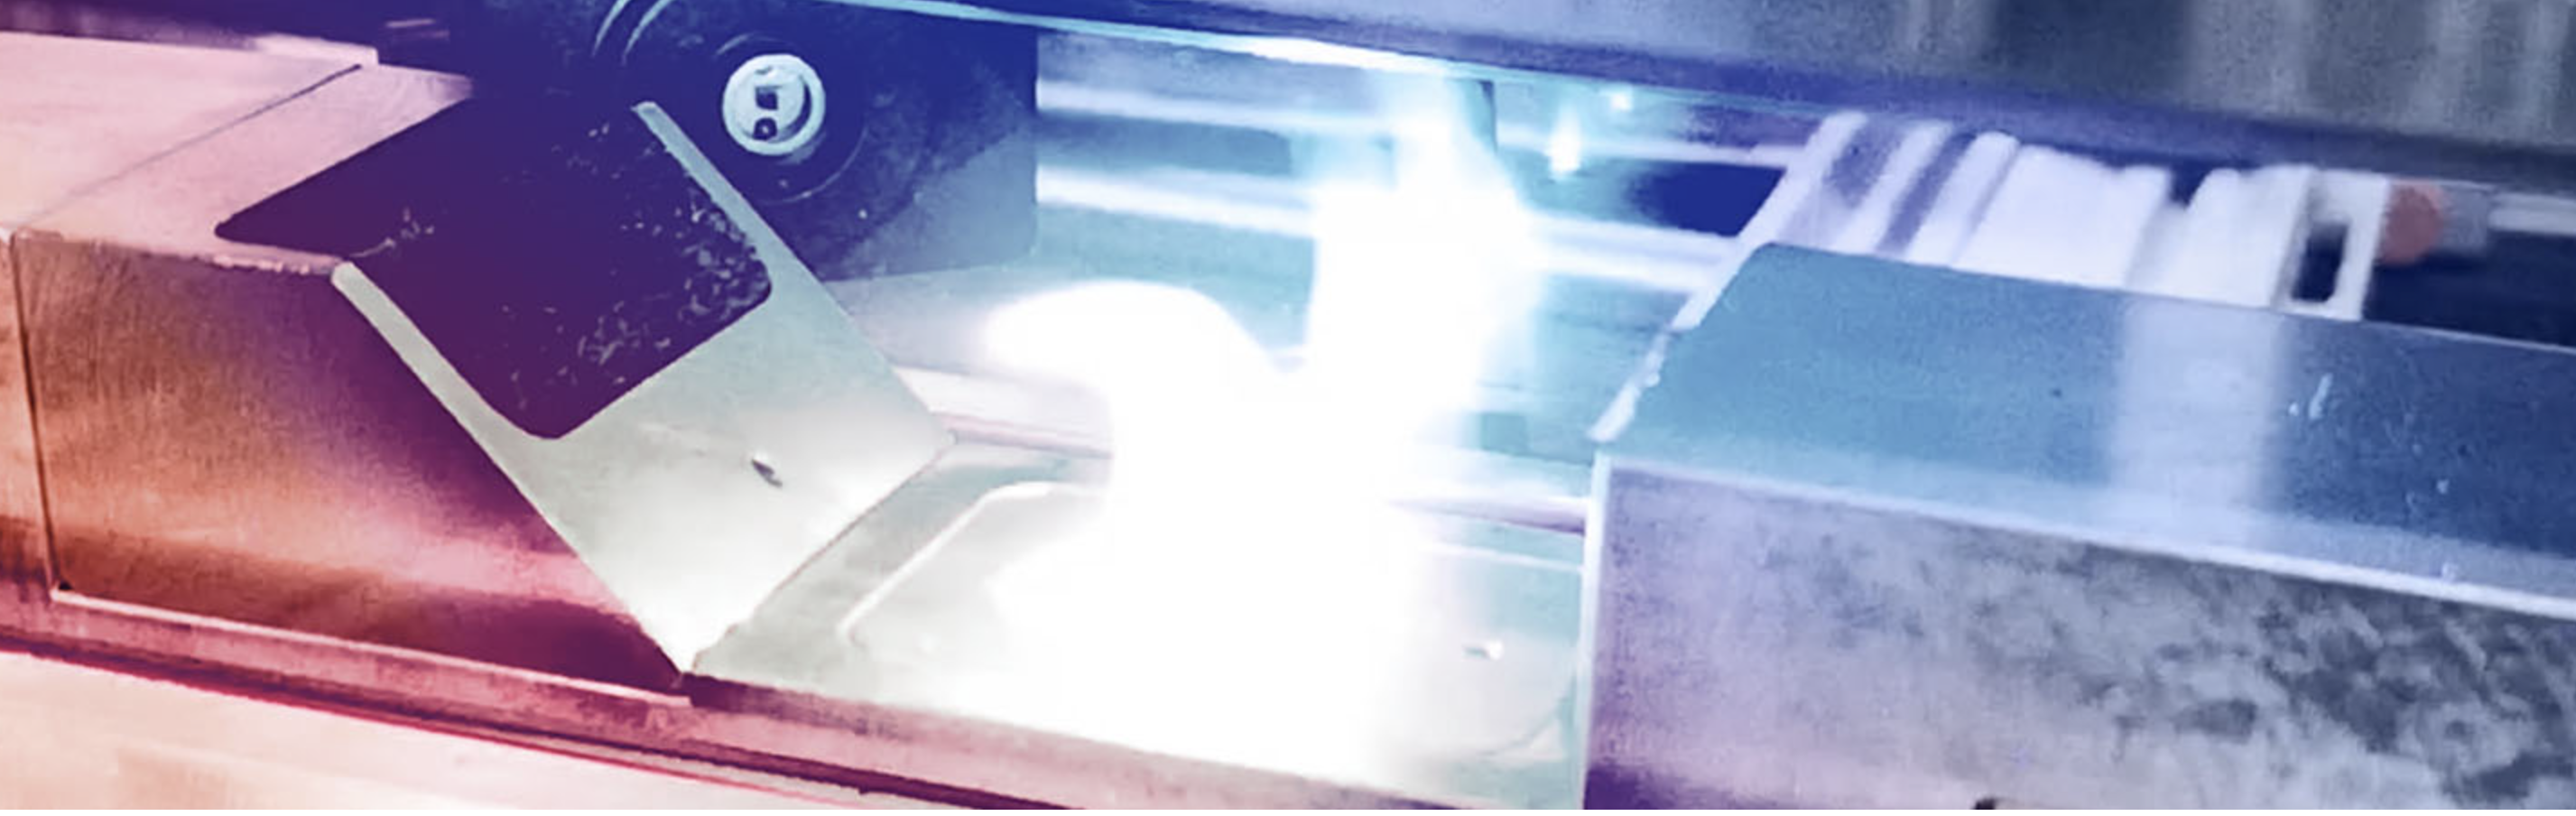
\includegraphics[width=\textwidth]{Figures/mtc/ceesd_actii.png}
\end{frame}

\begin{frame}\frametitle{Novel Composite Scramjets}



\begin{itemize}
\item \sPI{scramjet} --- \underline{the} technology for air-breathing
  hypersonics propulsion

\item Employ high-$T$ composite materials to advance designs

\begin{center}
\begin{minipage}{0.45\textwidth}
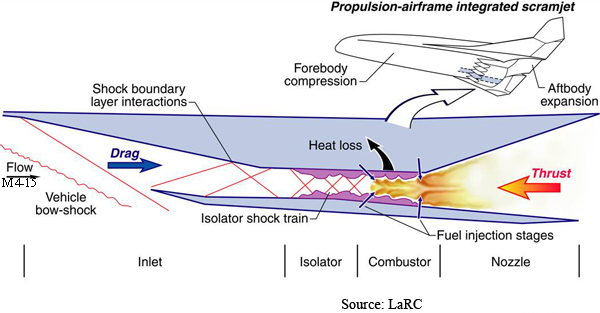
\includegraphics[width=\textwidth]{Figures/scramjet-LaRC.png}
\end{minipage}
\hfil
\begin{minipage}{0.45\textwidth}
\raisebox{0.3in}{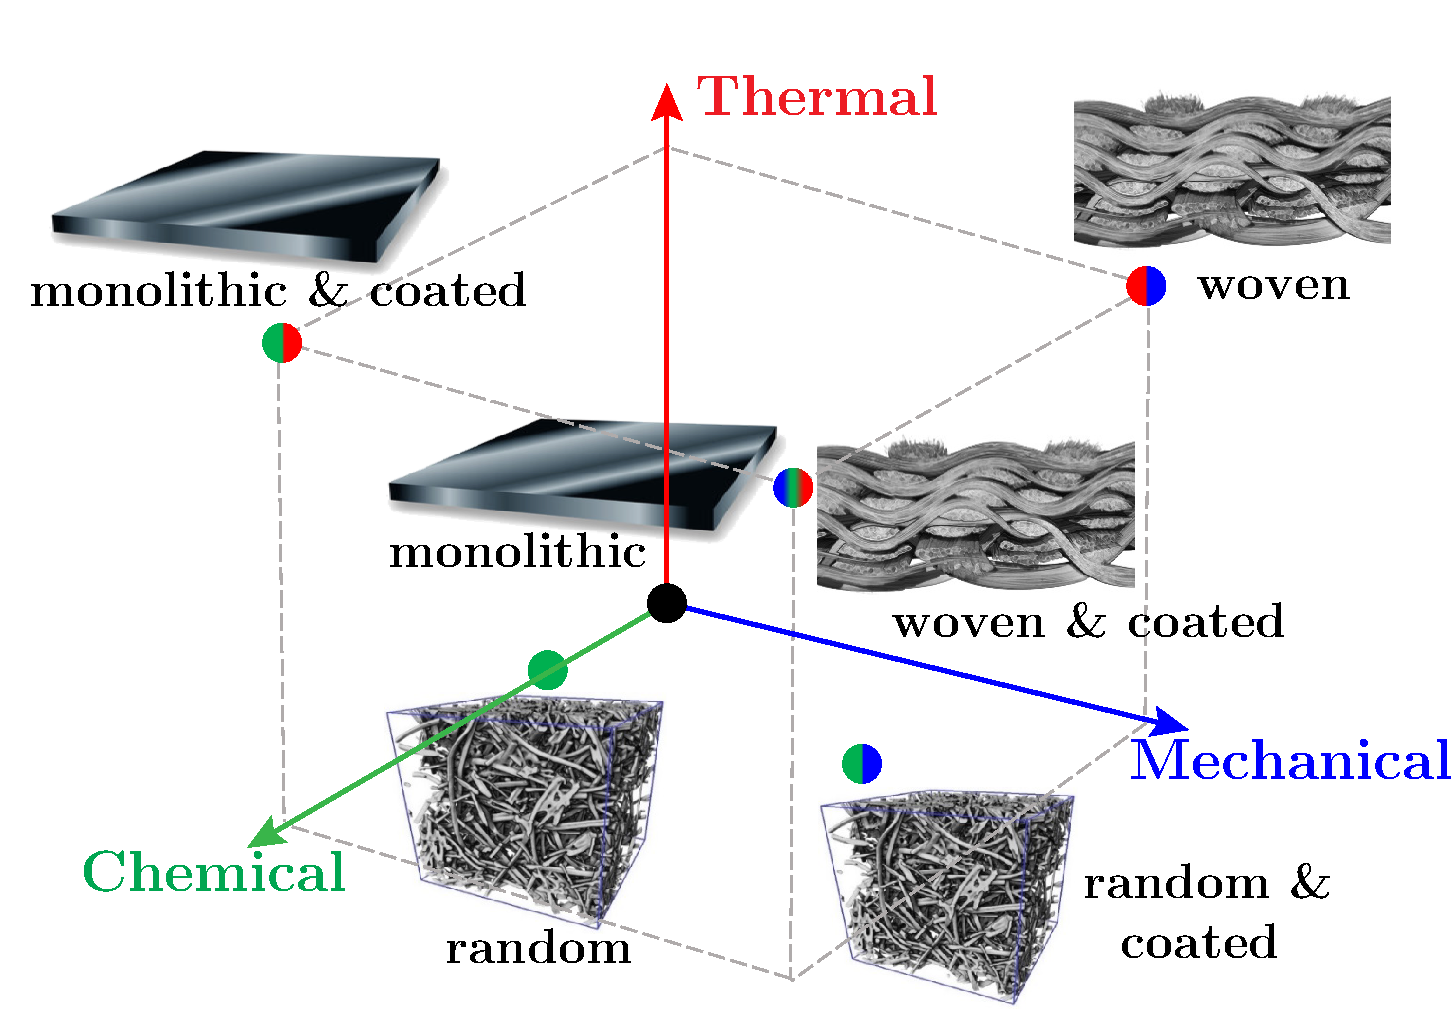
\includegraphics[width=\textwidth]{Figures/composite-design.pdf}}
\end{minipage}
\end{center}


  \item \rPI{Predictions}:  avoid costly/prohibitive testing,
    accelerate design and innovation

\end{itemize}

\end{frame}

\begin{frame}\frametitle{Experimental Facilities \prj{\tiny}{Lee}}


\vspace*{0.15in}
\begin{itemize}
\setlength{\itemsep}{0.in}
\item \cPI{ACT-II}:  on-campus AFOSR-funded supersonic combustion facility


%\begin{center}
\includegraphics[width=0.55\textwidth]{Figures/actii-y0-setup.pdf}
%\end{center}
\insertmovie{0.3}{y2-target.png}{y2-target.mov}

\item Arcjet driven: low cost ($\lesssim$ \$10), low turnaround
  time ($\lesssim$ 5\,min)

\item V\&V of integrated physics models and prediction

\item Additional experimental facilities: McKenna stand burner, Atomic Oxygen chamber, et al

\end{itemize}
%\hfil

\end{frame}
%======================================================================

\begin{frame}\frametitle{Integrated Center}

\begin{itemize}
\setlength{\itemsep}{0.22in}

\item CEESD is an integrated center, with computer
  scientists, computational scientists, and experimentalists working in concert

\end{itemize}

\begin{center}
  \onslide<1>{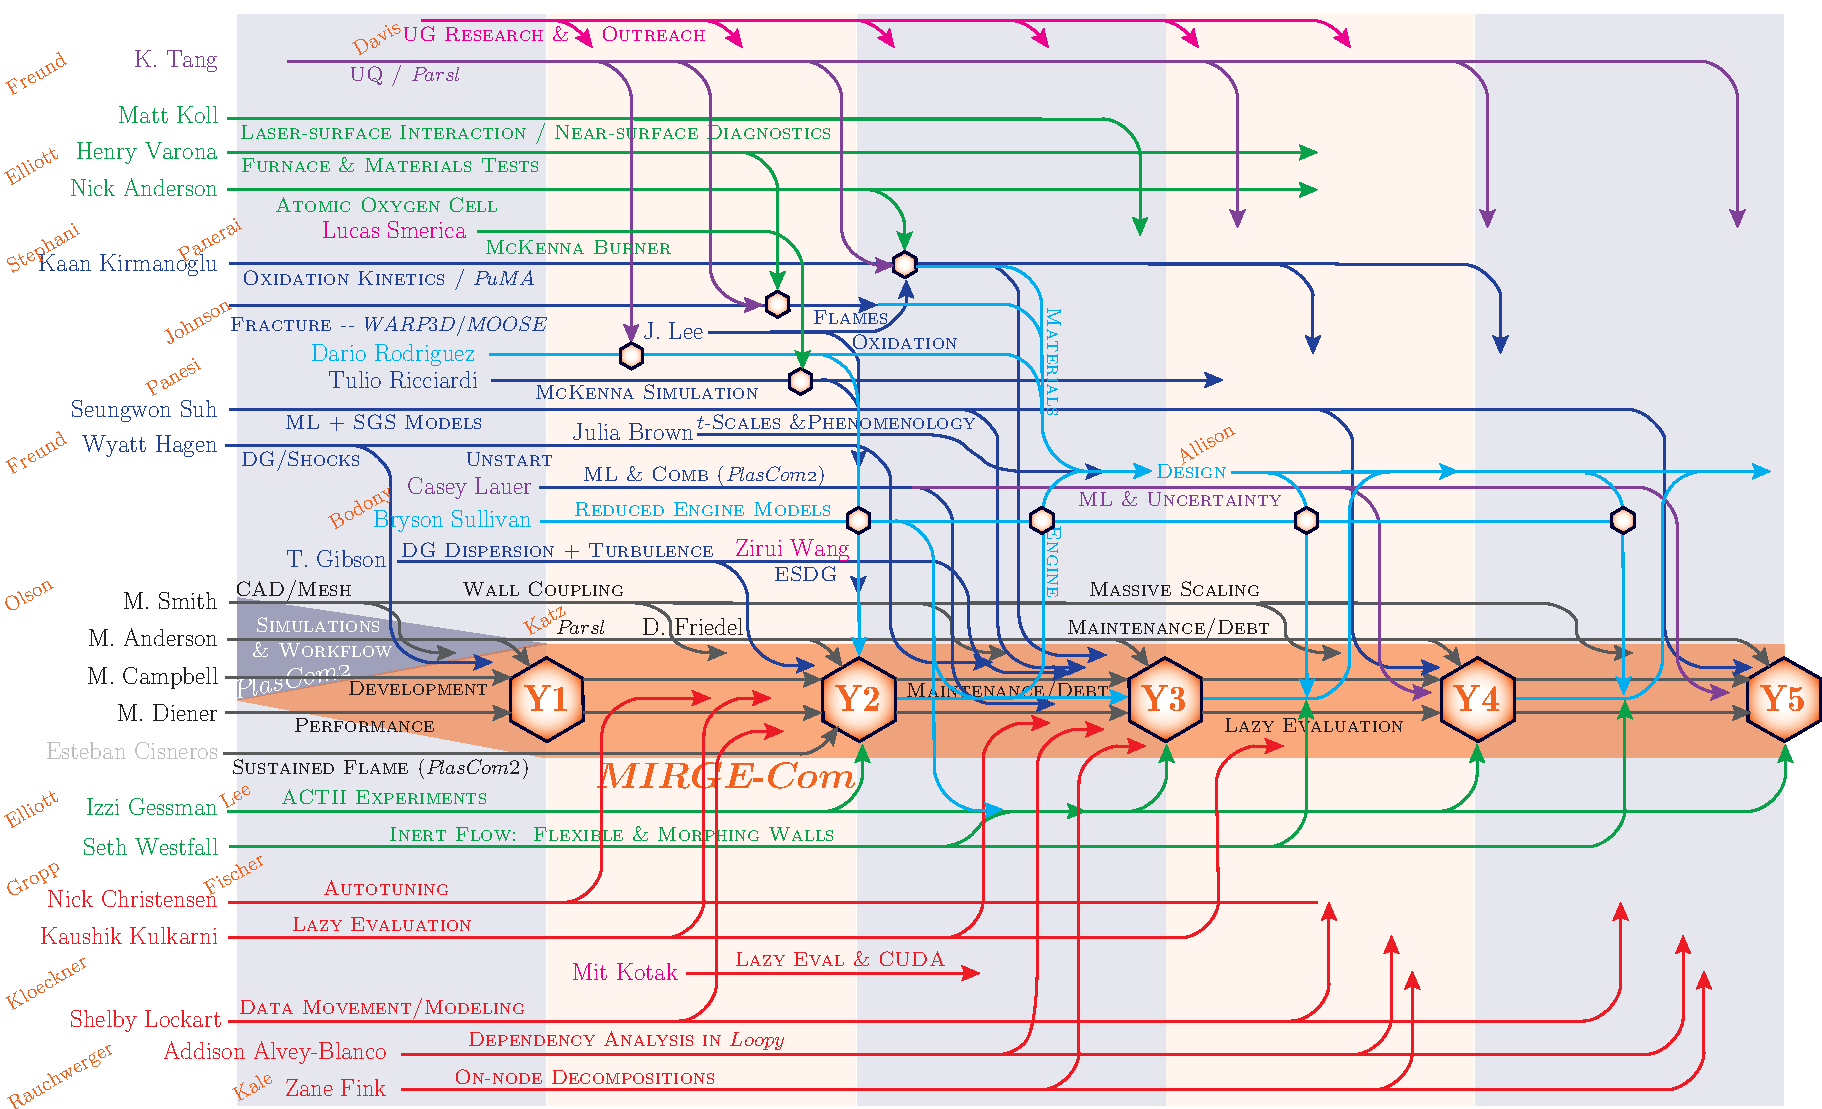
\includegraphics[width=0.65\textwidth]{Figures/ceesd-roadmap-review2022.pdf}}
\end{center}

\end{frame}

\begin{frame}\frametitle{Architecture Overview}
  \begin{center}
  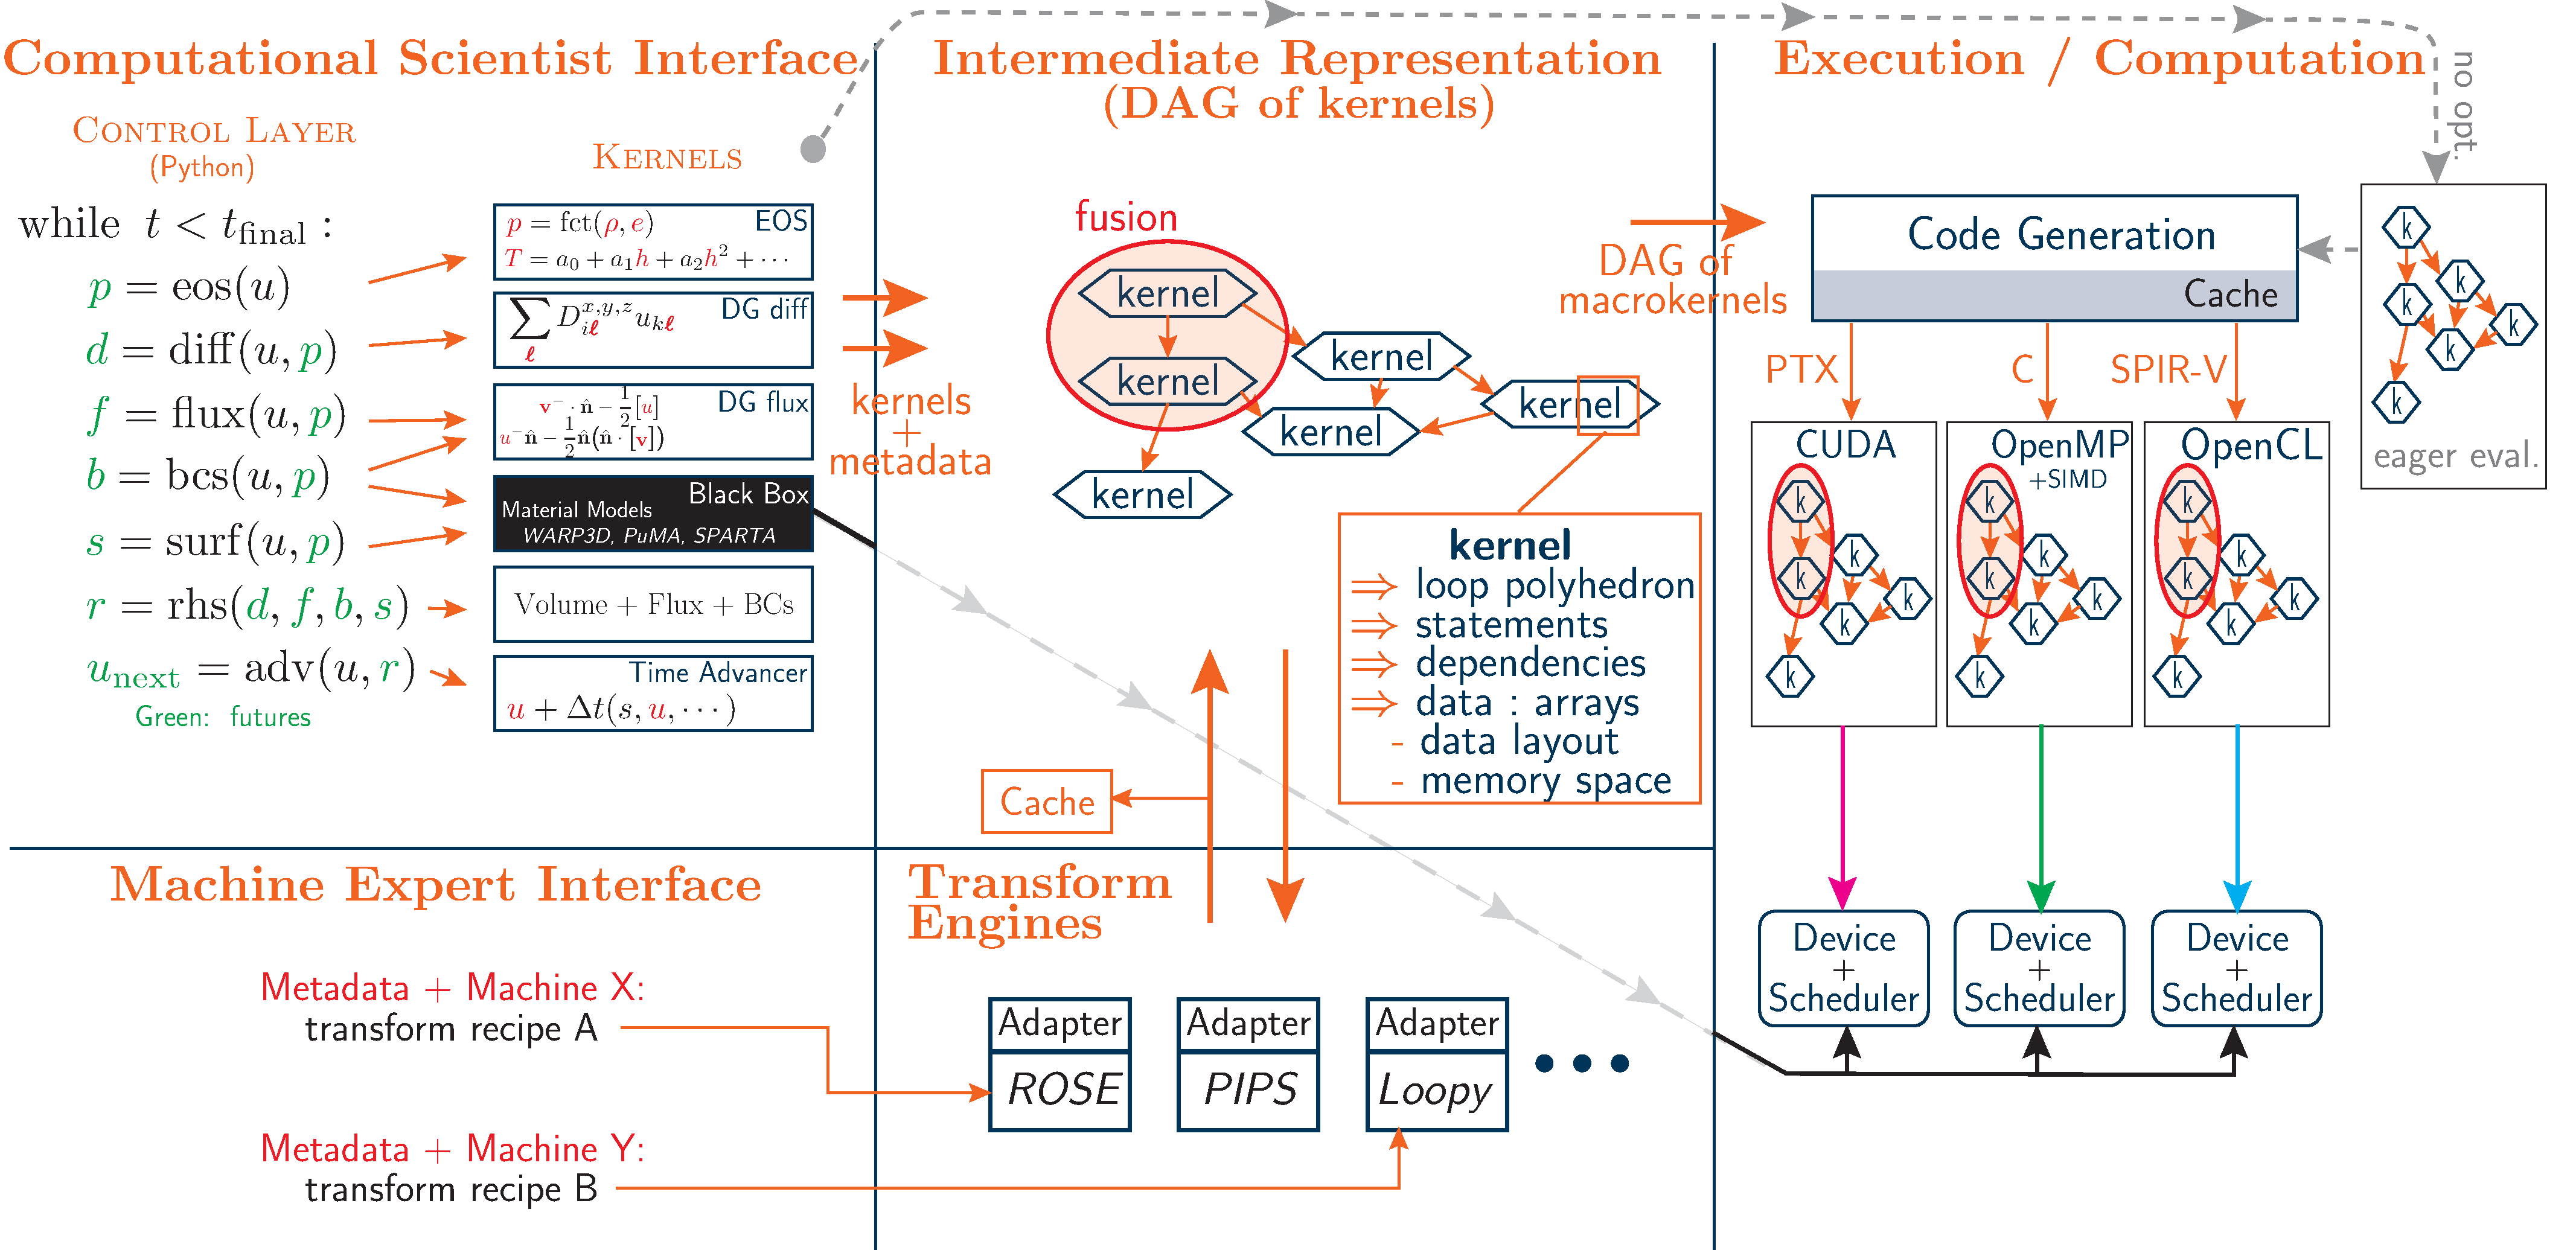
\includegraphics[width=.95\textwidth]{Figures/controllayer-new.pdf}
  % \vspace*{-5pt}
  \end{center}
\end{frame}

%======================================================================
\begin{frame}[t]\frametitle{CS Framework (MIRGE)}

\begin{center}
\onslide*<1>{\hspace*{-0.01\textwidth}\fcolorbox{myBlue}{white}{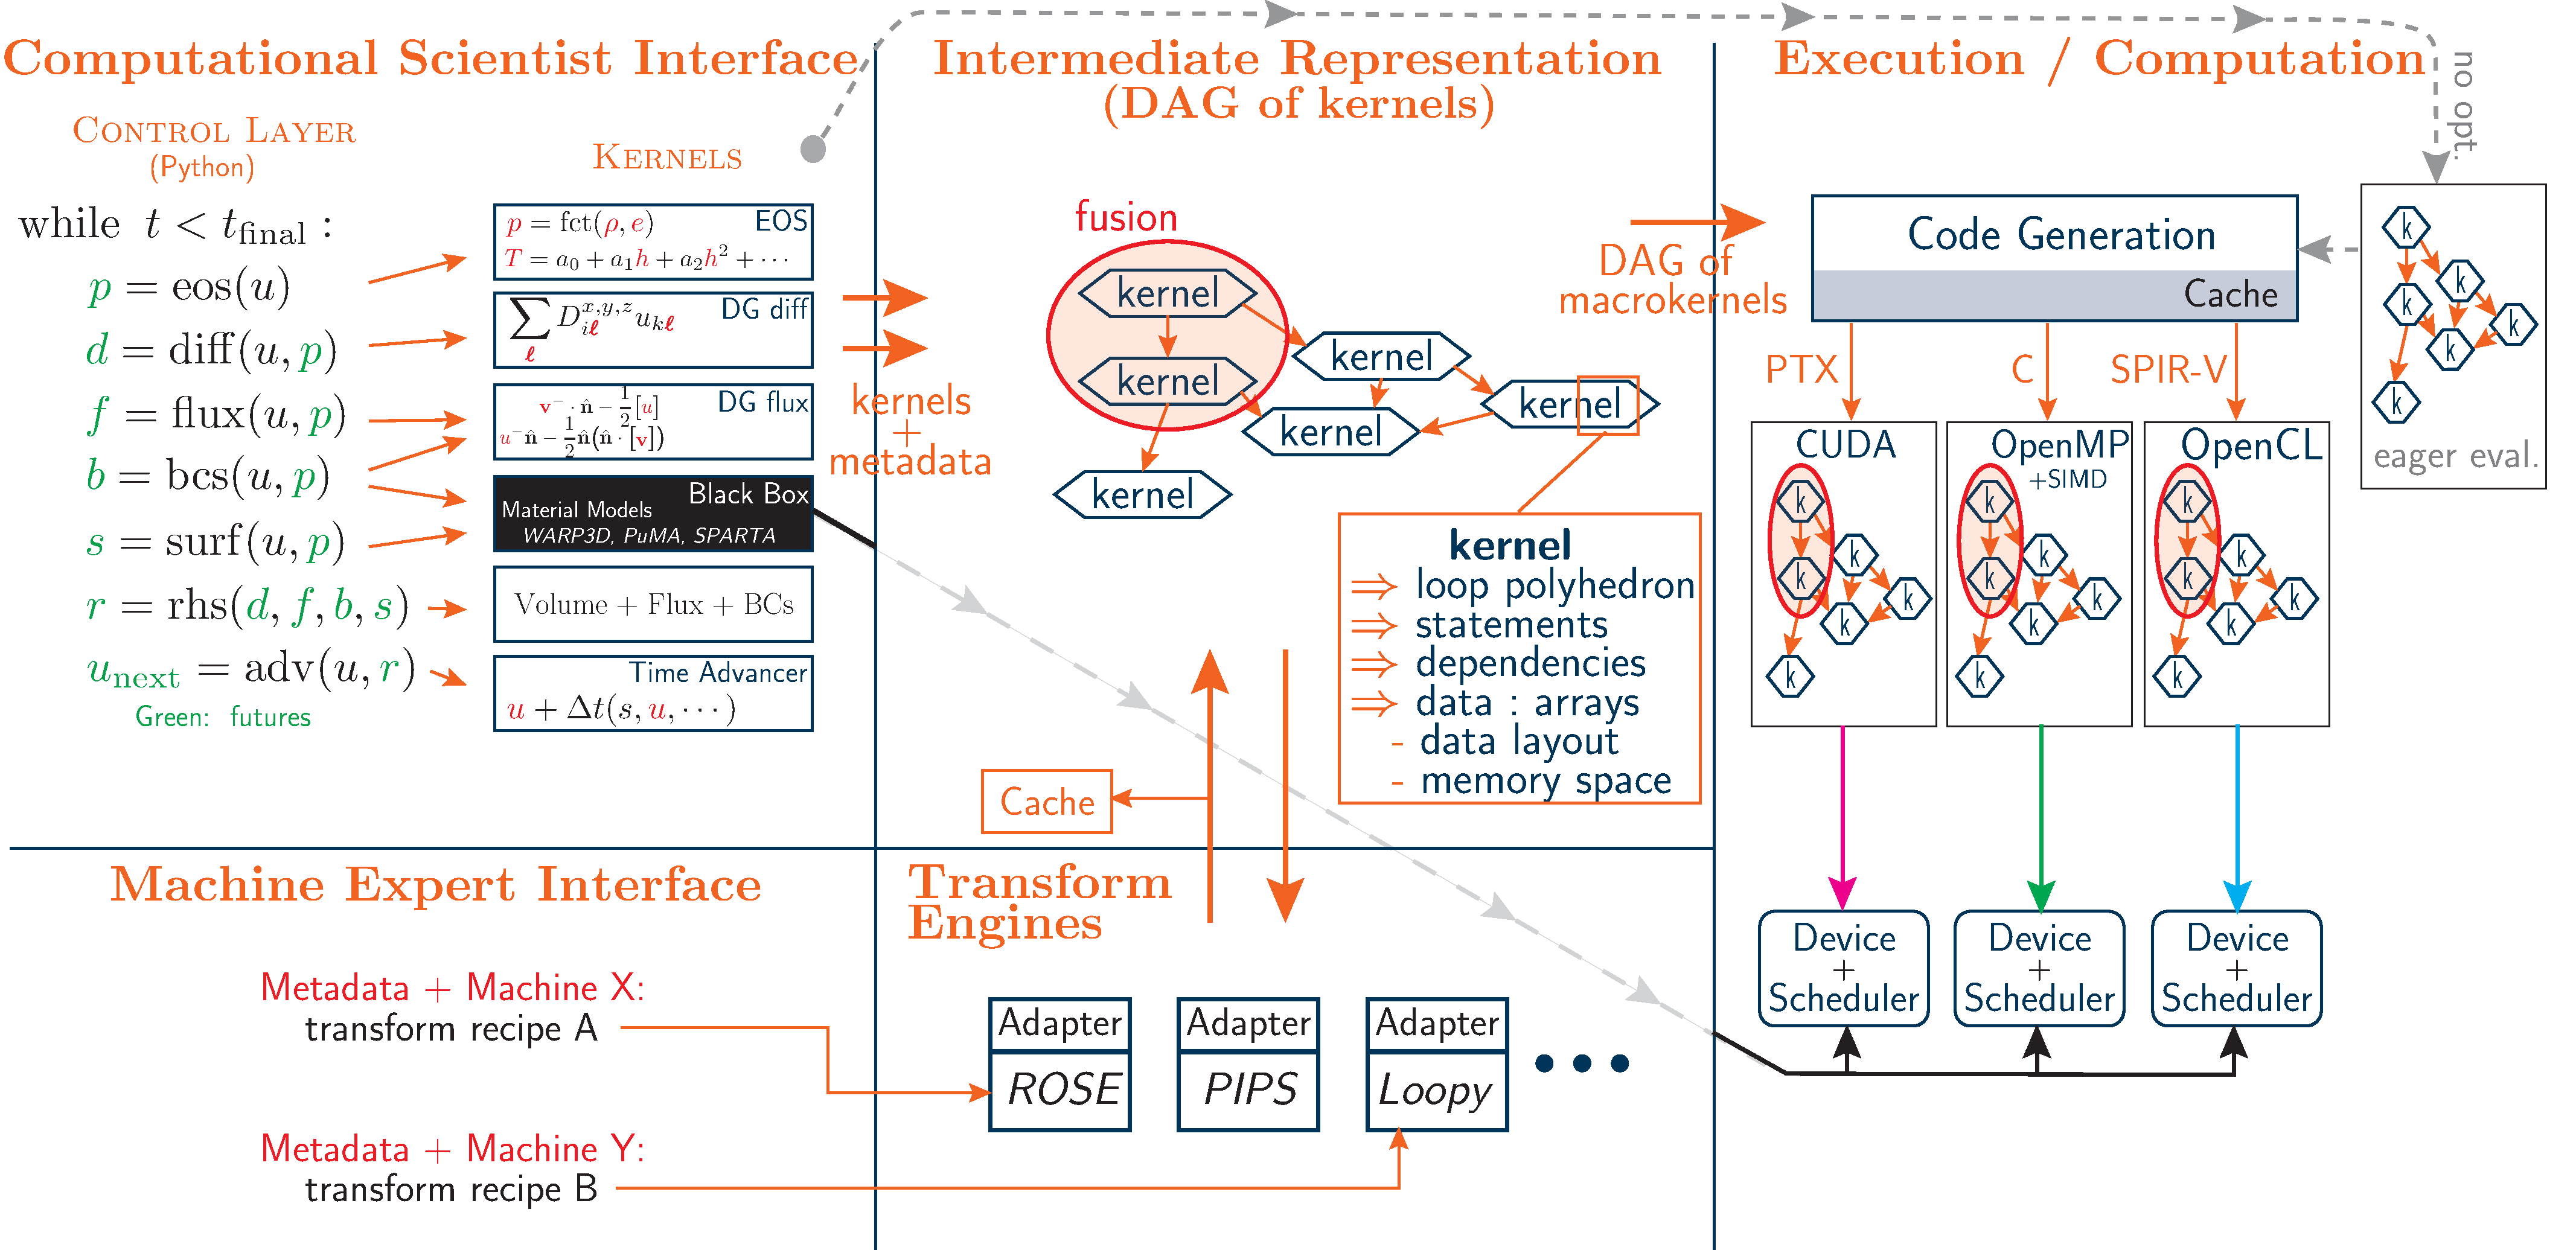
\includegraphics[width=0.75\textwidth]{Figures/controllayer-new.pdf}}}
\onslide*<2>{\hspace*{-0.01\textwidth}\fcolorbox{myBlue}{white}{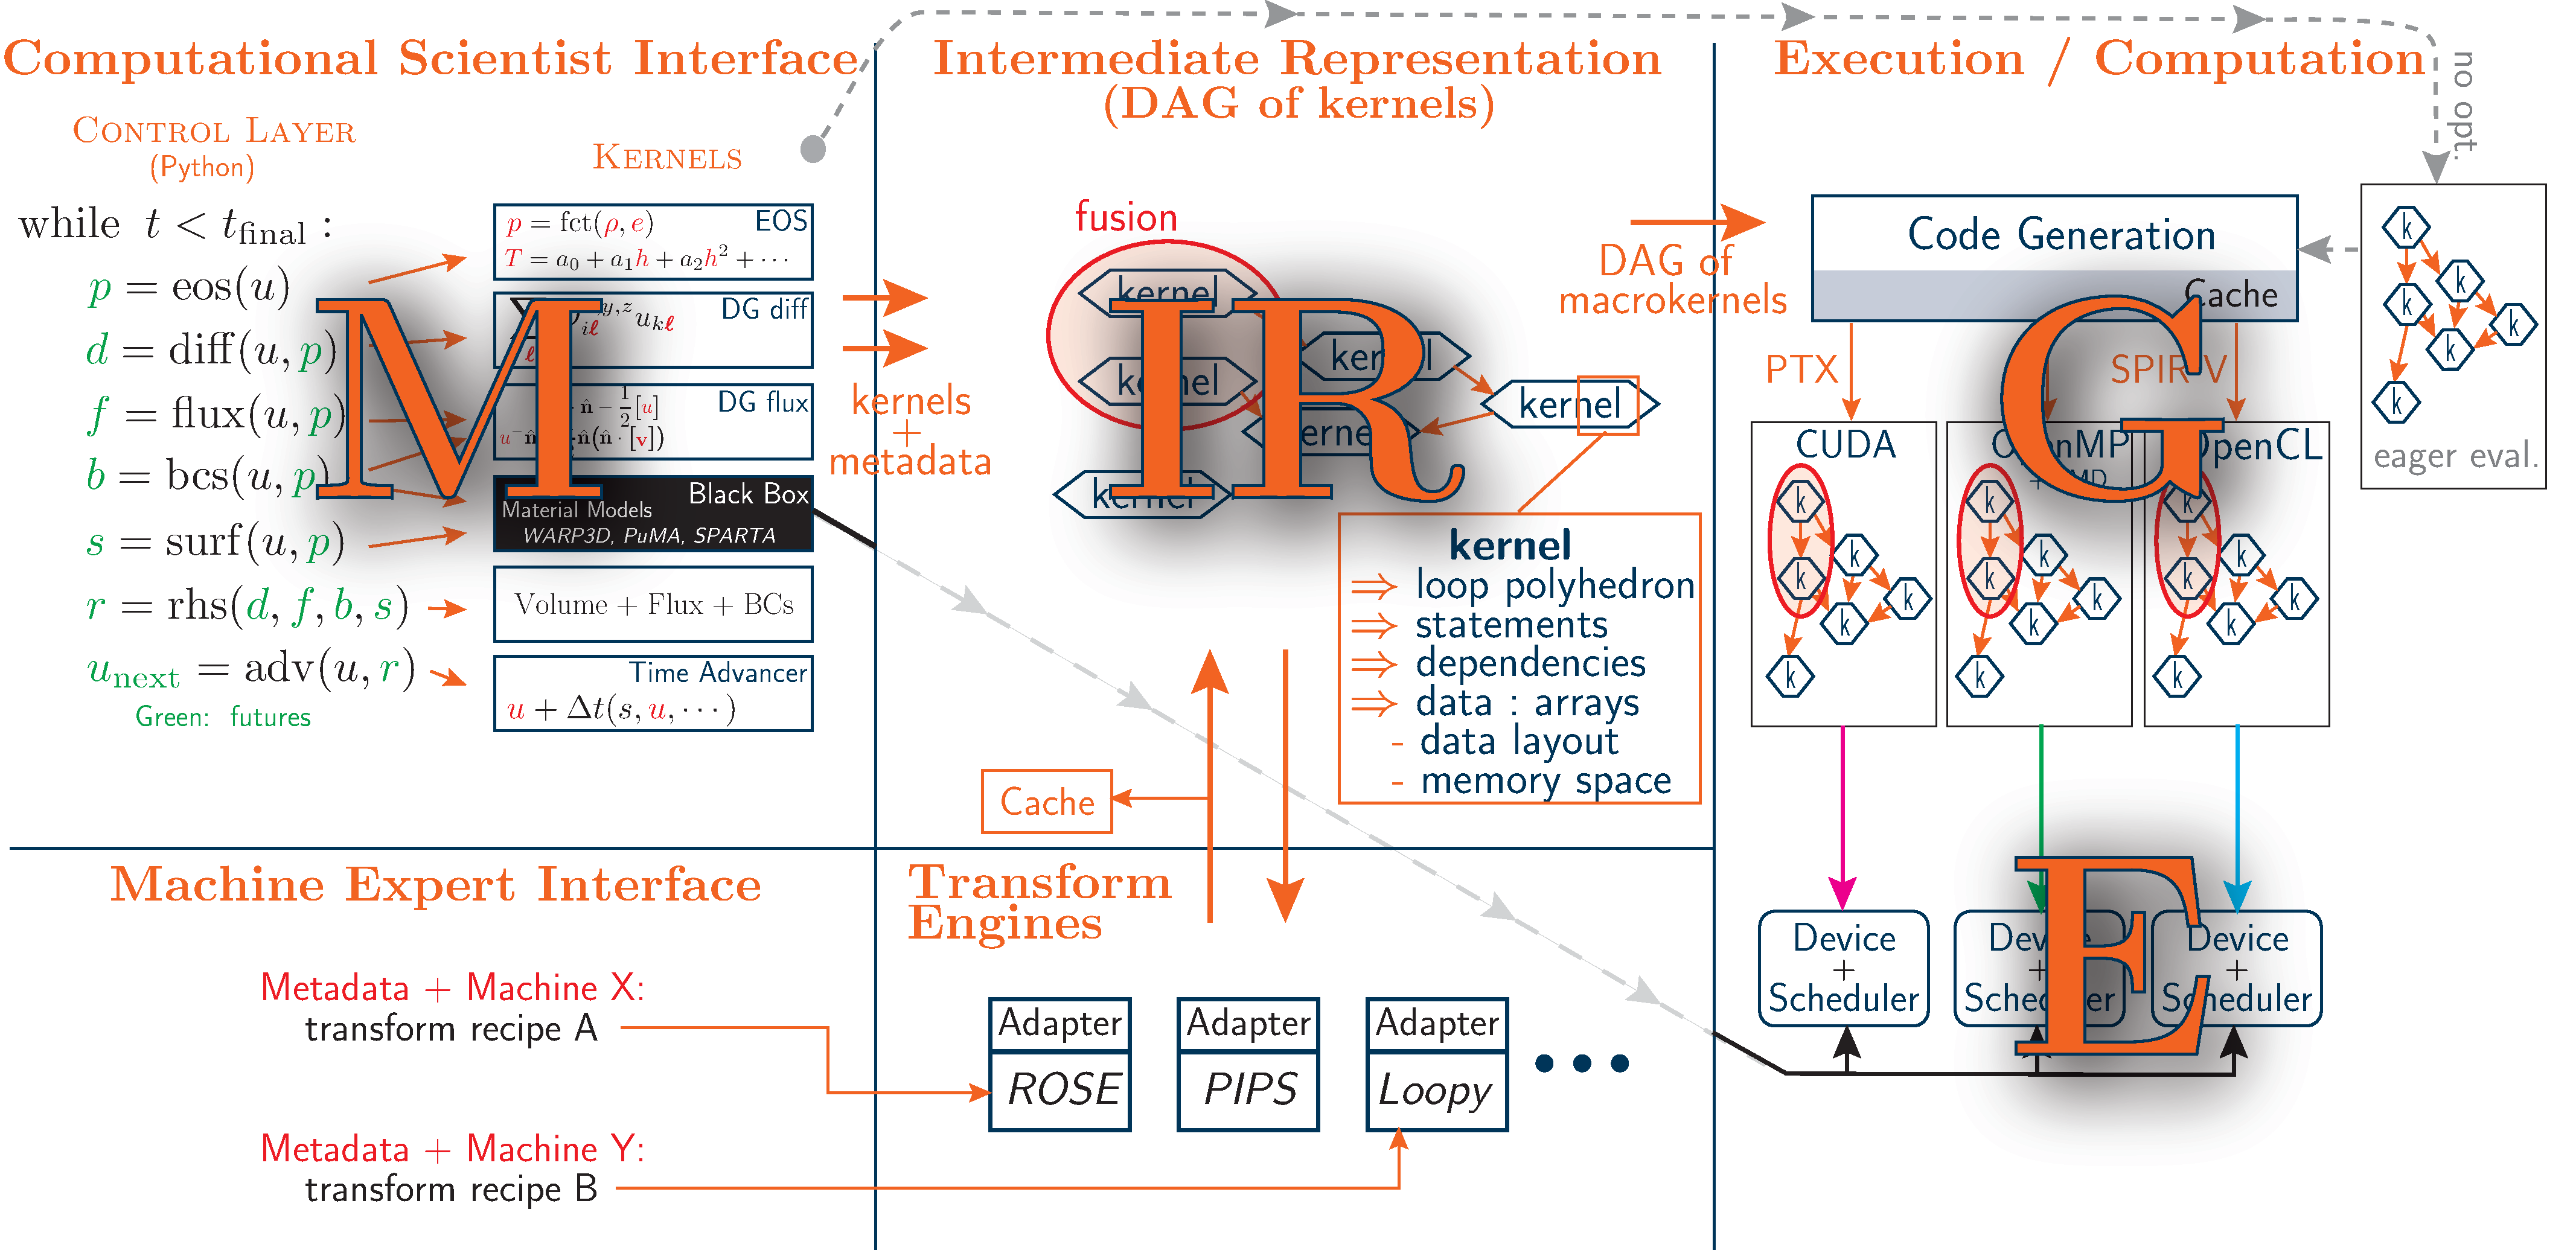
\includegraphics[width=0.75\textwidth]{Figures/controllayerMIRGE-new.pdf}}}

\vspace*{0.1in}
\onslide*<2>{\textbf{\cPI{M}ath $\cdot$ \cPI{I}ntermediate
    \cPI{R}epresentation $\cdot$ \cPI{G}eneration $\cdot$
    \cPI{E}xecution}
\vspace*{0.1in}

\cPI{MIRGE} approach $\Rightarrow$ simulations with
\iPI{MIRGE-Com}

}


\end{center}

\end{frame}
%======================================================================

%======================================================================
\begin{frame}\frametitle{\ceesdcode{}
    \prj{\tiny}{M.~Anderson, M.~Campbell, M.~Smith, Olson,
      Freund, Kl\"ockner}}

%  \begin{minipage}{0.3\textwidth}
%    \huge \cPI{\ceesdcode{}}
%  \end{minipage}
%  \hfill
  \begin{minipage}{0.65\textwidth}
    \begin{itemize}
      \setlength{\itemsep}{0.1in}
    \item Discontinuous Galerkin (DG)
      \vspace*{-0.04in}
      \begin{itemize}
      \item localize computational intensity
      \item unified BC formulation
      \item unstructured for complex and changing geometries
      \item leverage experience \prj{\tiny}{Fischer, Olson,
          Kl\"ockner}
      \item concerns:  resolution, dissipation\xnew
      \end{itemize}
    \item Feature complete for Y3 
      \vspace*{-0.04in}
      \begin{itemize}
      \item Compressible Navier--Stokes
      \item Combustion chemistry
      \item Multi-species gas-phase EOS, transport
      \item Species limiting, shock
        capturing (new Y2) 
      \item 2-way coupled $T$ and \ce{O2} transport in ``wall'' (new Y2)
      \item Surface radiation (new Y3)\xnew
        \prj{\tiny}{M.~Smith, 04, T.~Ricciardi, 07b}
      \item Porous phenolic material (new Y3)\xnew
        \prj{\tiny}{T.~Ricciardi, 07b}
      \end{itemize}
    \item Developed entirely in CEESD's \ceesdMIRGE{} framework
%    \item Piecewise for performance \ldots   
    \end{itemize}
  \end{minipage}
  \hfill
  \begin{minipage}{0.34\textwidth}
     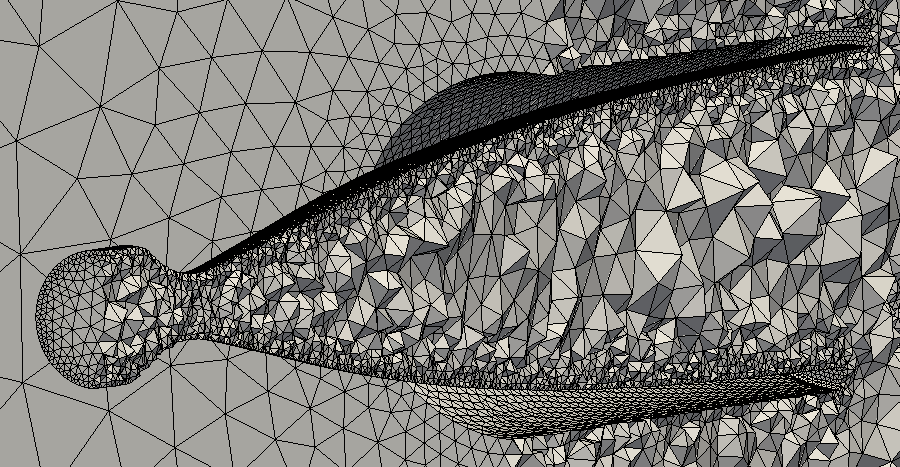
\includegraphics[width=\textwidth]{Figures/nozzle-mesh.png}
     \par\noindent
     \vspace*{25pt}
     \phantom{\rule{\textwidth}{0.5pt}} % Invisible rule to ensure spacing
     \insertmovie{1.05}{fluid-smith.png}{y2-2d.mov}
%     \includegraphics[width=\textwidth]{Figures/}
  \end{minipage}
%  \hfill
\vspace{-15pt}
\begin{center}
https://github.com/illinois-ceesd/mirgecom
\end{center}
\end{frame}


\begin{frame}\frametitle{Main Challenge - DAG Size and Complexity}
\vspace{10pt}
\begin{minipage}[t][0.4\textheight][t]{\textwidth}
\begin{multicols}{2}
\begin{itemize}
\item \textit{DAG Splat}: Flux DAG inlined for element boundary treatment
\item DAG for each rank neighbor
\item DAG for each BC
\end{itemize}
\columnbreak
\begin{table}
\centering
%\caption*{Simulation DAG Node Counts}
\begin{tabularx}{\linewidth}{|X|X|X|X|X|}
\hline
\textbf{Gas} & \textbf{Vol} & \textbf{BC} & \textbf{IEB} & \textbf{Total} \\ \hline
Single & 290 & 486 & 697 & 1473 \\ \hline
Mixture & 1591 & 2500 & 3060 & 7151 \\ \hline
\end{tabularx}
%\vspace{10pt}
$N_{\text{dag}} = 1591 + 2500(N_{\text{bc}}) + 3060(1 + N_{\text{pb}})$
%\begin{tabular}{|l|r|r|r|r|}
%\hline
%\textbf{Gas model} & \textbf{Volume} & \textbf{Wall BC} & \textbf{Inter-element Boundary} & \textbf{Total} \\ \hline
%Single gas & 290 & 486 & 697 & 1473 \\ \hline
%Mixture & 1591 & 2500 & 3060 & 7151 \\ \hline
%\end{tabular}
\end{table}
\end{multicols}
\end{minipage}\vfill
\vspace{-20pt}
\begin{minipage}[t][0.4\textheight][t]{\textwidth}
\centering
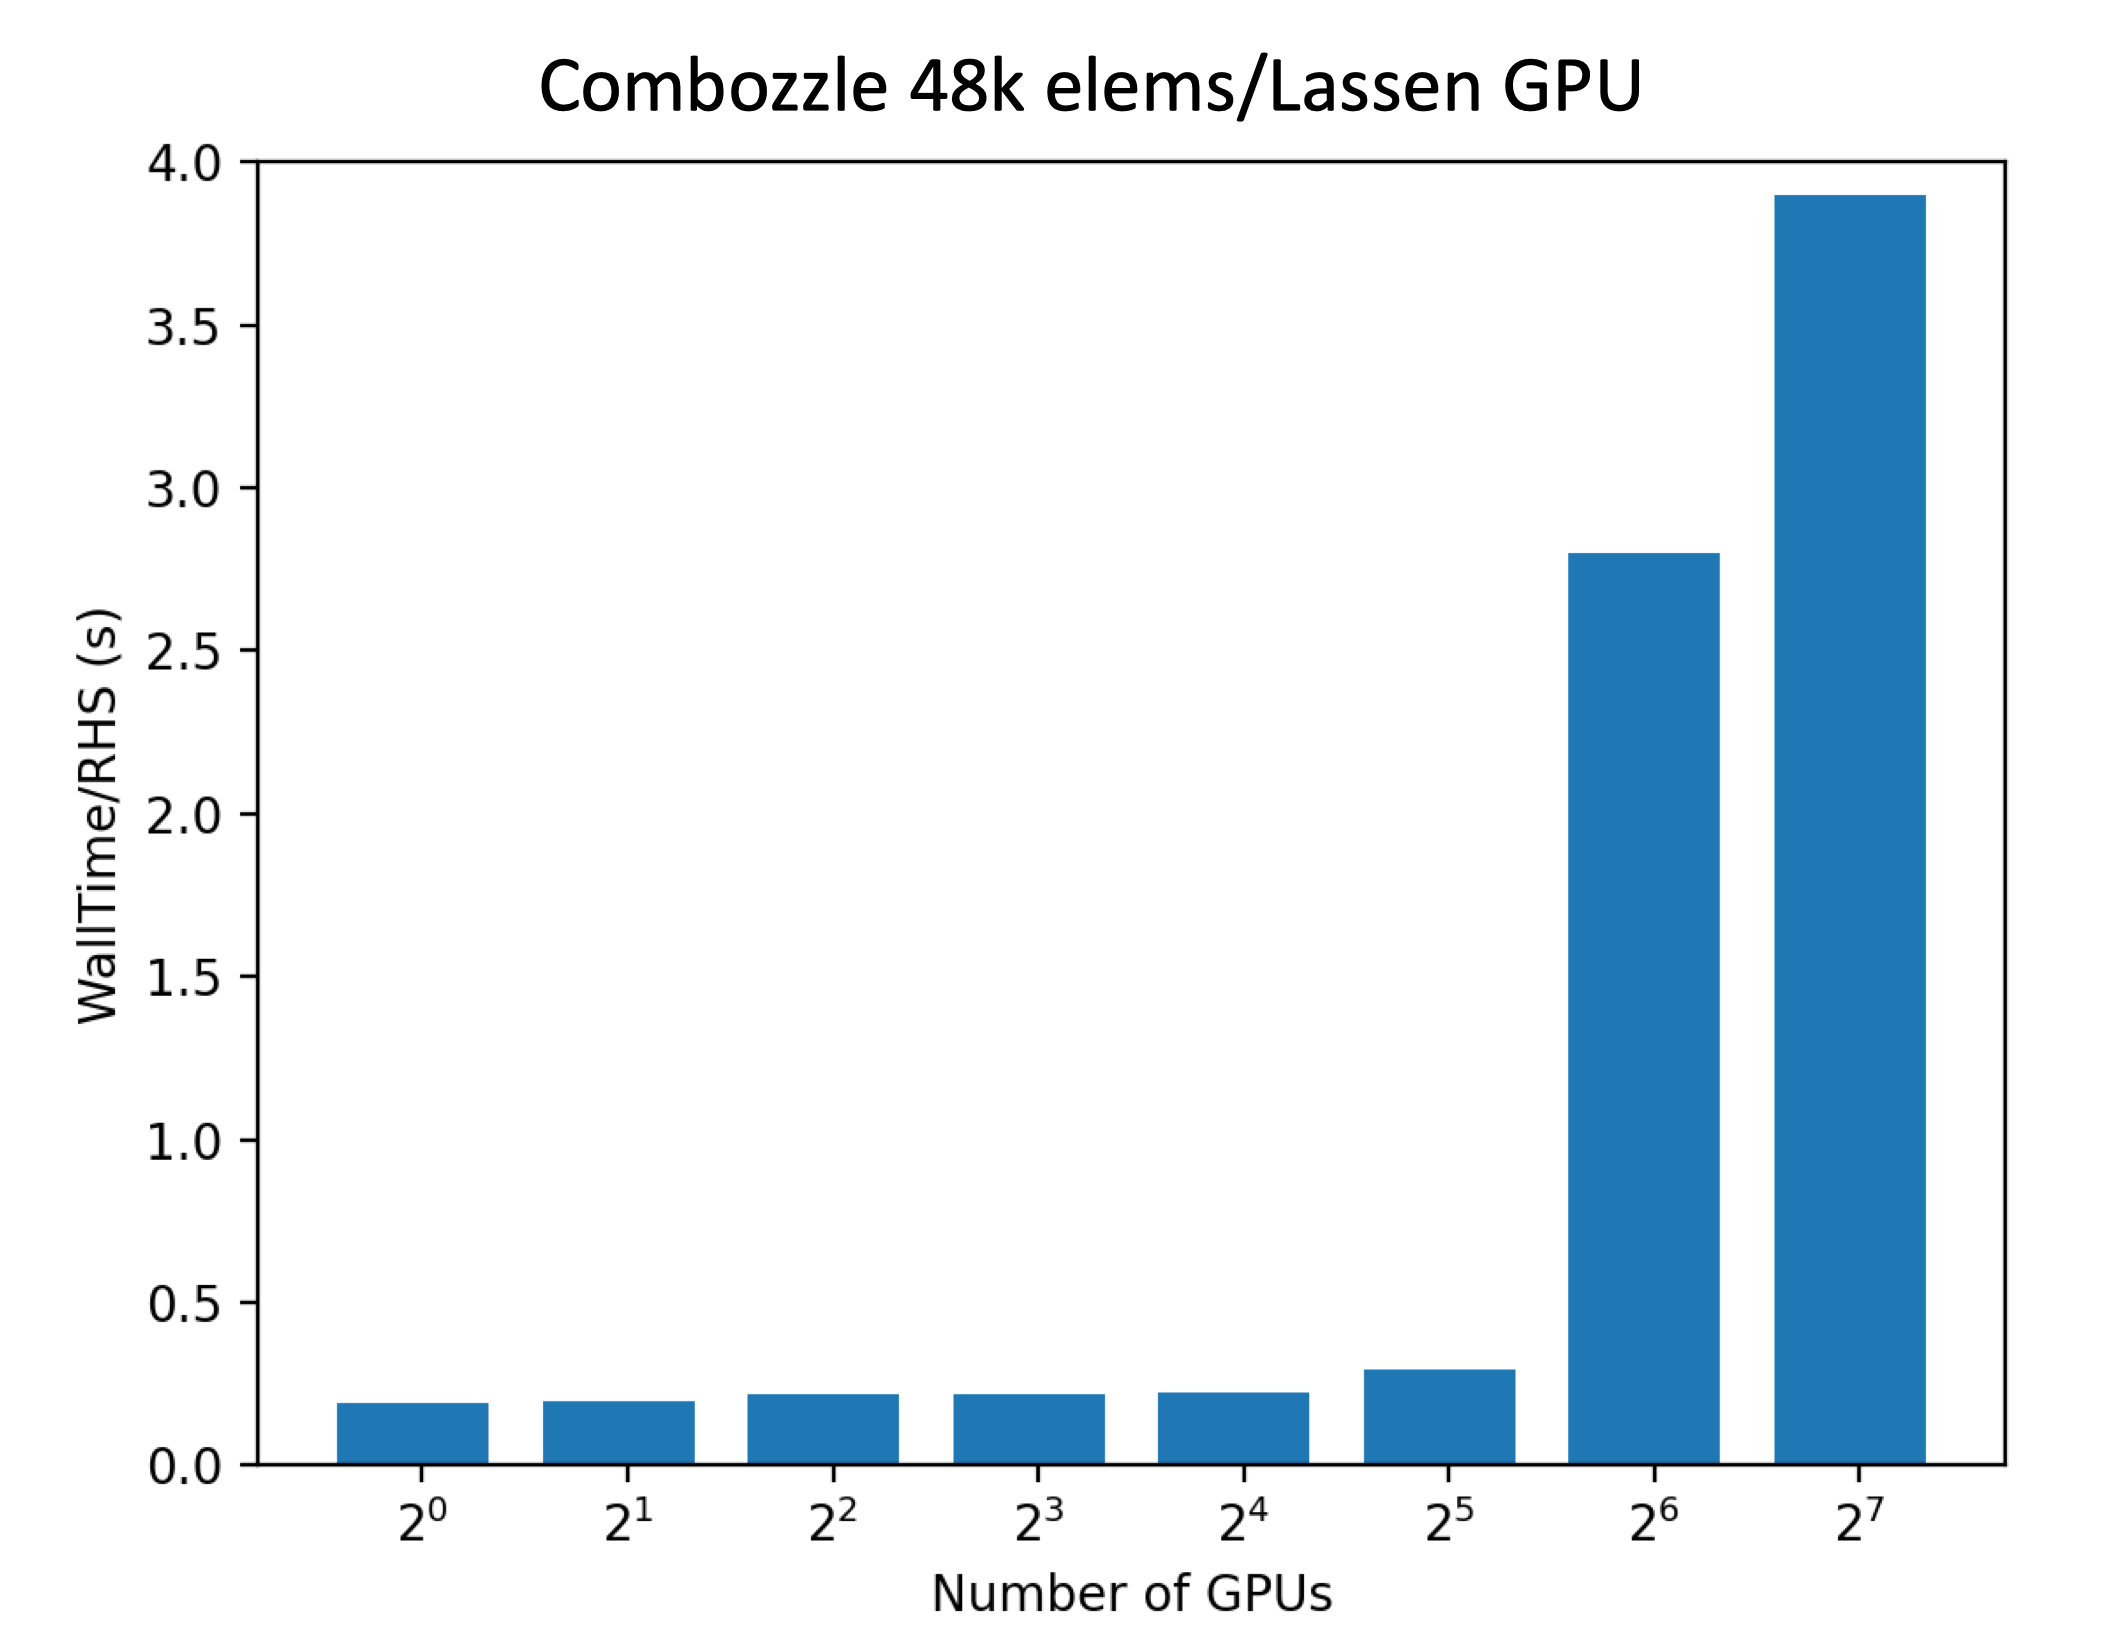
\includegraphics[width=.4\textwidth]{Figures/mtc/combozzle_weak_bad_partitioning.png}\hspace{30pt}
\vspace{-20pt}
%Sample box partitioning with Metis
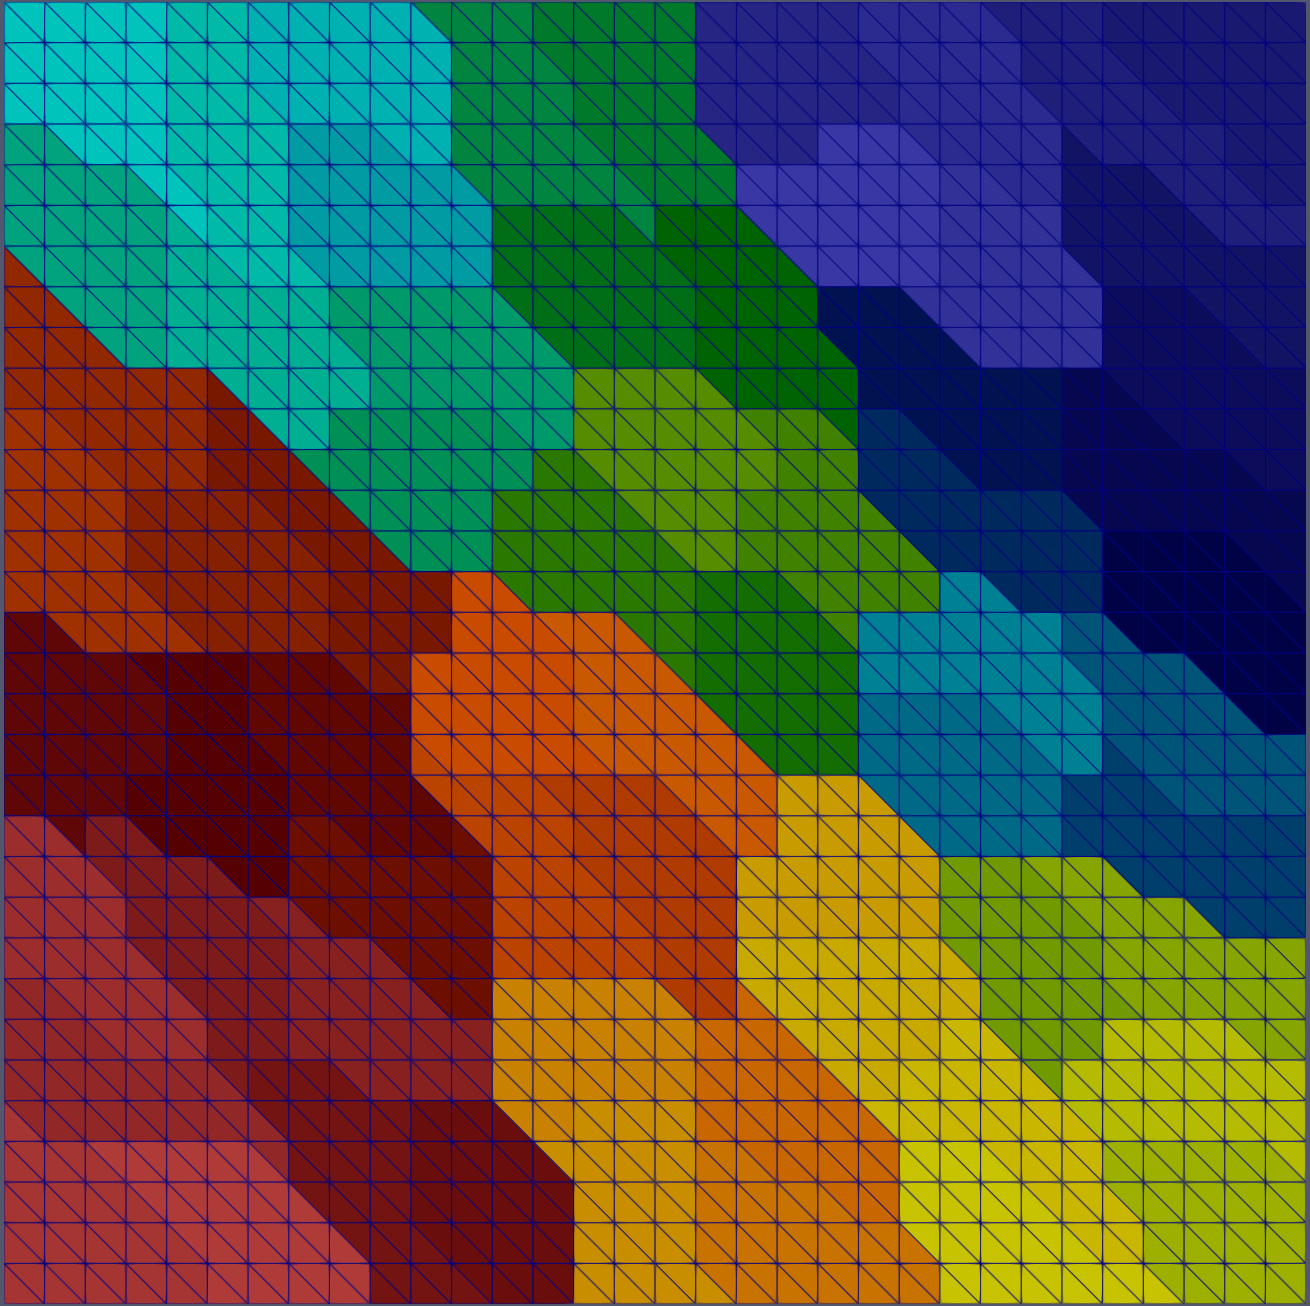
\includegraphics[width=.3\textwidth]{Figures/np64_part.png}
%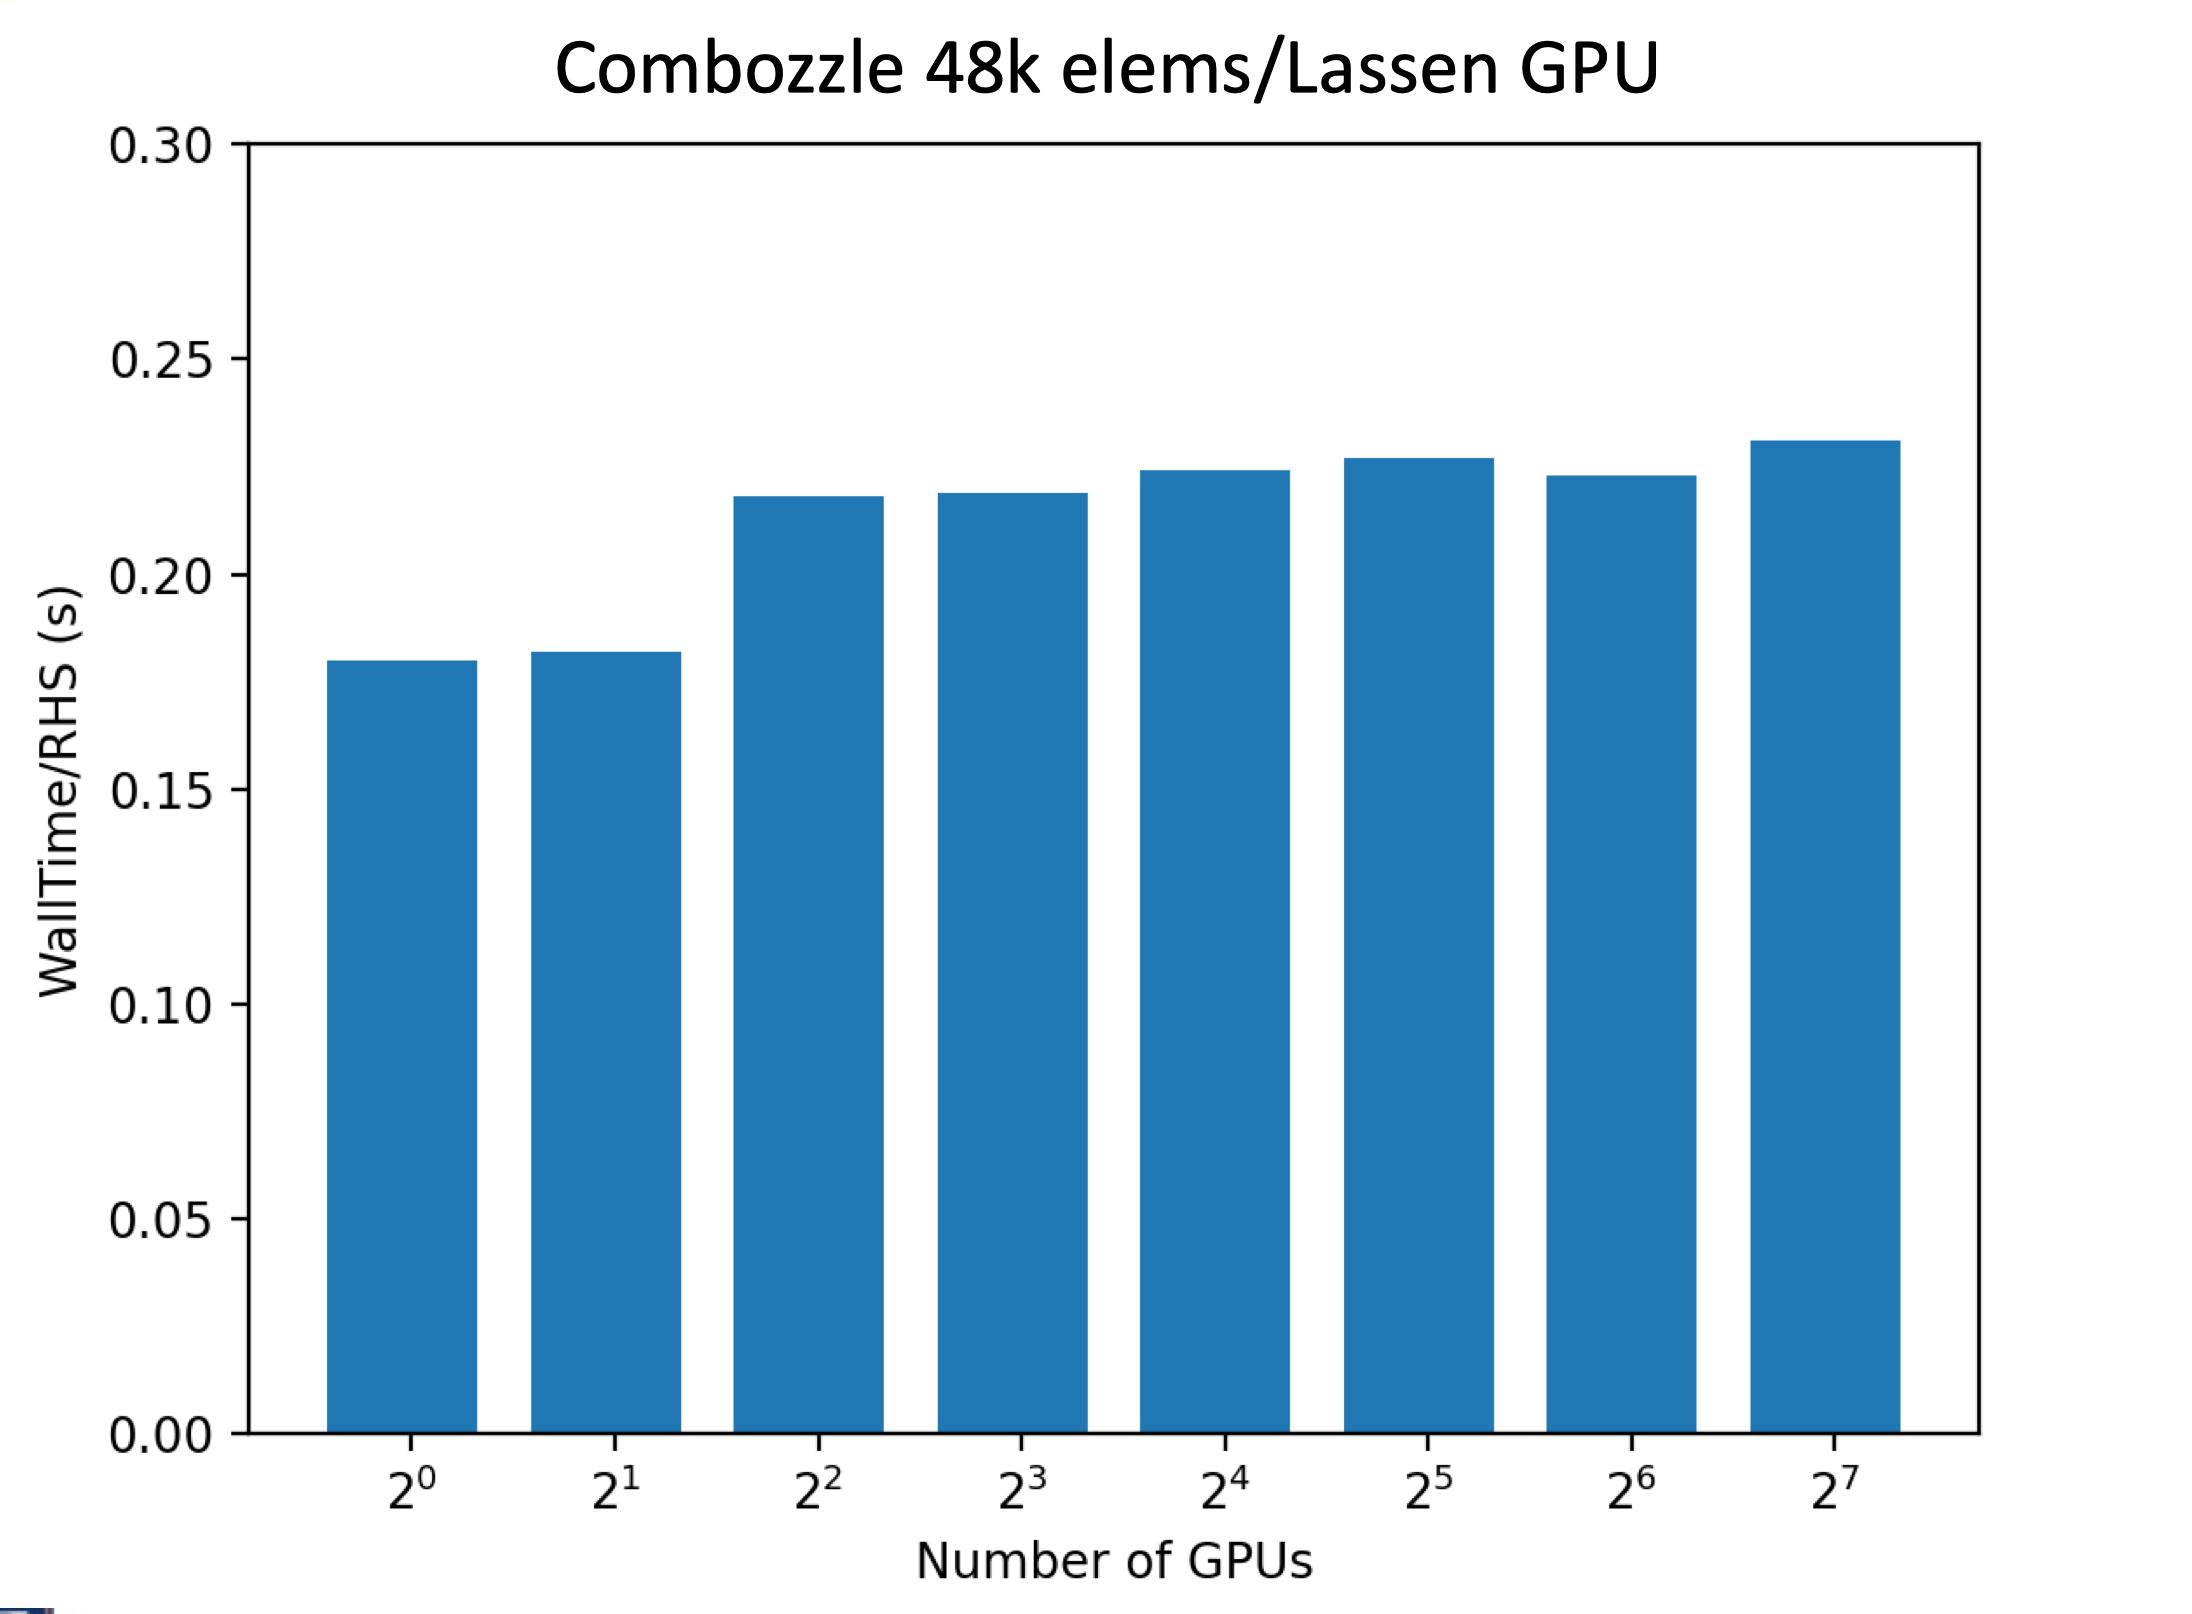
\includegraphics[width=.4\textwidth]{Figures/mtc/combozzle_weak_sliced_partitioning.png}
\end{minipage}
\end{frame}

\begin{frame}\frametitle{DAG Splat Mitigation}
\begin{minipage}[t][0.4\textheight][t]{\textwidth}
%\begin{center}
%New: prediction-enabling performance
%\end{center}
\begin{multicols}{2}
%\vspace{30pt}
\rule{0pt}{20pt}
\begin{itemize}
\setlength{\itemsep}{0pt} % Removes space between items
\setlength{\parskip}{0pt} % Removes space between paragraphs within an item
\setlength{\topsep}{0pt} % Removes space before and after the list
\item Mitigation: Metis vs. 1D decomp (pancakes)
\item Rank neighbors limited to 2
\item Unlocks prediction-scale simulation
\item Fixed, \sout{once and for all!} temporarily
\item Real, permanent solution: Function outlining
\end{itemize}
\columnbreak
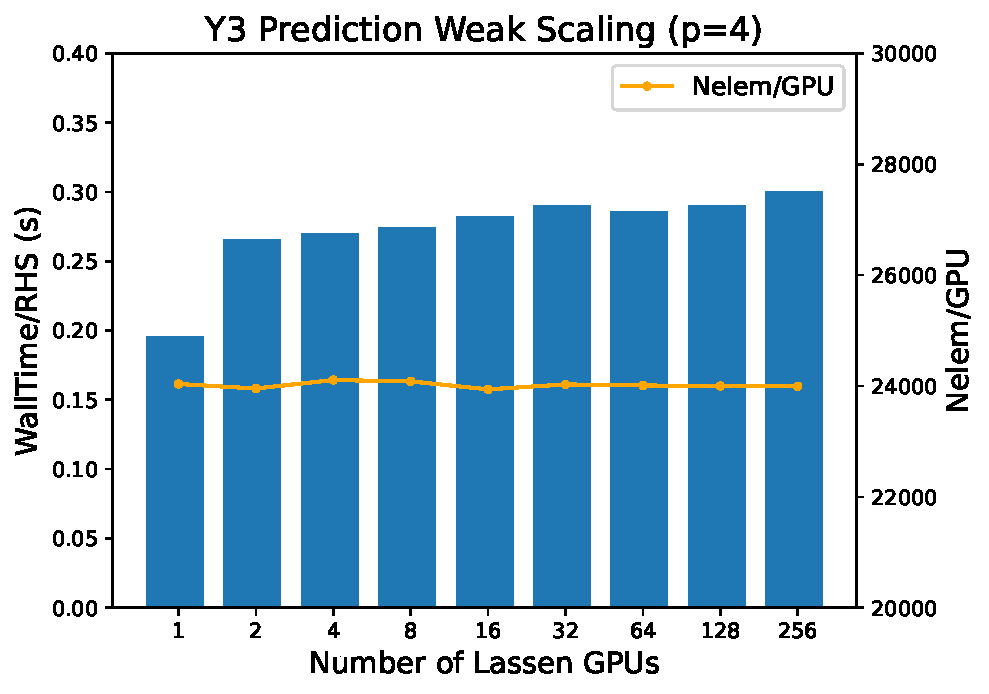
\includegraphics[width=.43\textwidth]{Figures/mtc/y3-prediction_weak_scaling.pdf}
\end{multicols}
\end{minipage}\vfill
%\vspace{-100pt}
\begin{minipage}[t][0.4\textheight][t]{\textwidth}
\centering
%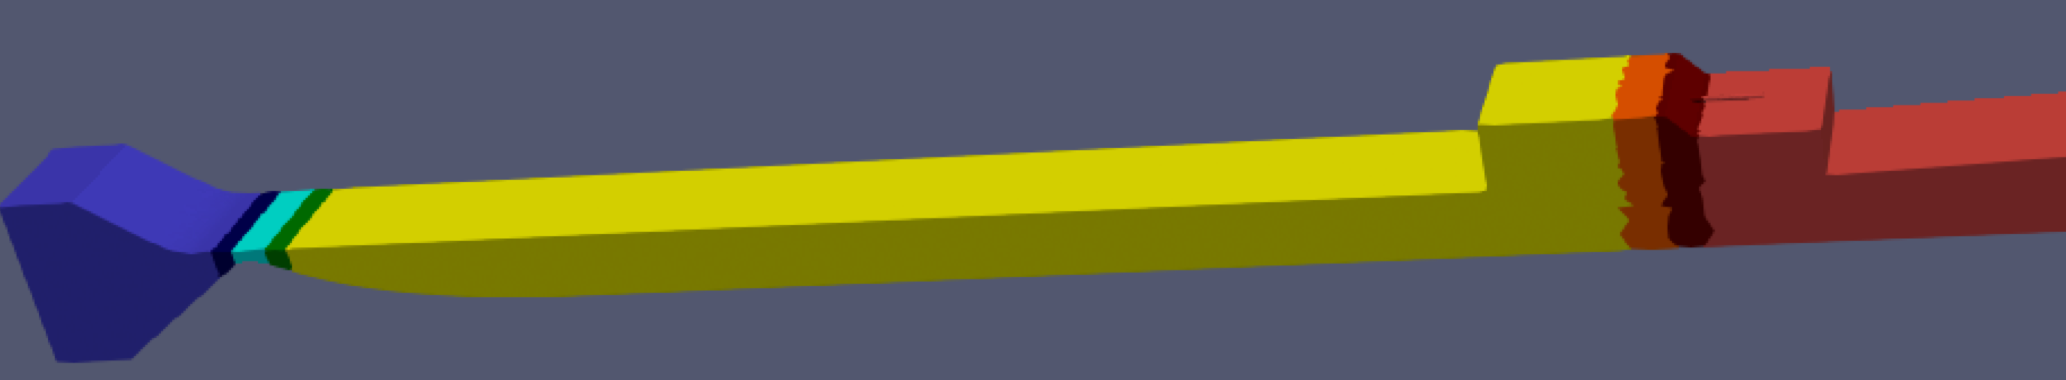
\includegraphics[width=.9\textwidth]{Figures/mtc/1dpart_bal.png}\\
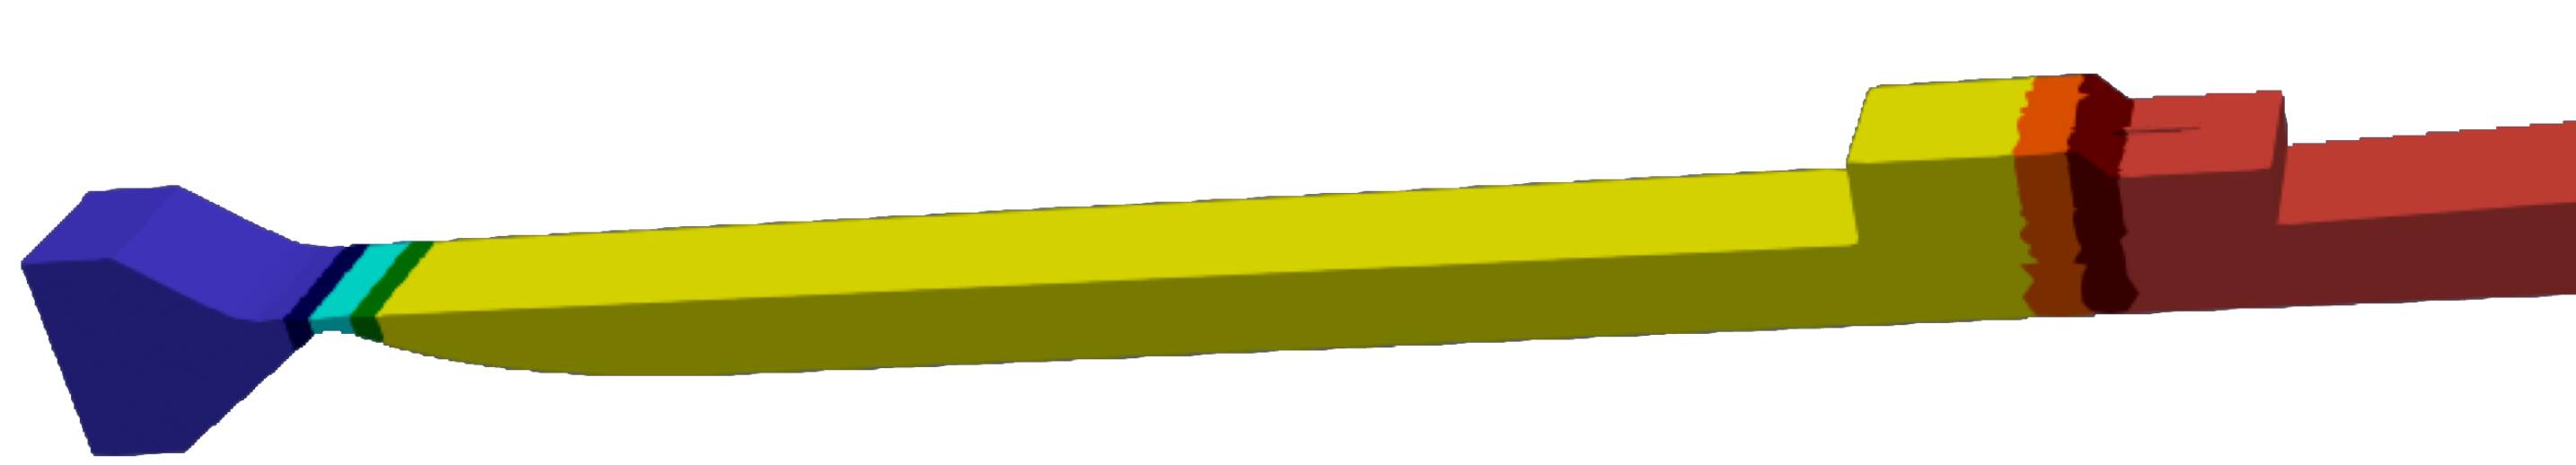
\includegraphics[width=.9\textwidth]{Figures/mtc/1dpartshiny.png}\\
%\vspace{-50pt}
\begin{center}
Prediction Domain Decomposition
\end{center}
\end{minipage}
\end{frame}

%\begin{frame}\frametitle{Scaling with 1D Partitioning}
%\begin{minipage}[t][0.4\textheight][t]{\textwidth}
%\begin{center}
%New: prediction-enabling performance
%\end{center}
%\begin{multicols}{2}
%\begin{itemize}
%\item Mitigation: Metis vs. 1D decomp
%\item Rank neighbors limited to 2
%\item Unlocks prediction-scale simulation
%\columnbreak
%\item Real fix: Function calls in the DAG (a.k.a. outlining)  \prj\tiny{M.~Smith}% \prj\tiny{Kaushik Kulkarni}
%\end{itemize}
%\end{multicols}
%\end{minipage}\vfill
%\vspace{-20pt}
%\begin{minipage}[t][0.4\textheight][t]{\textwidth}
%\centering
%%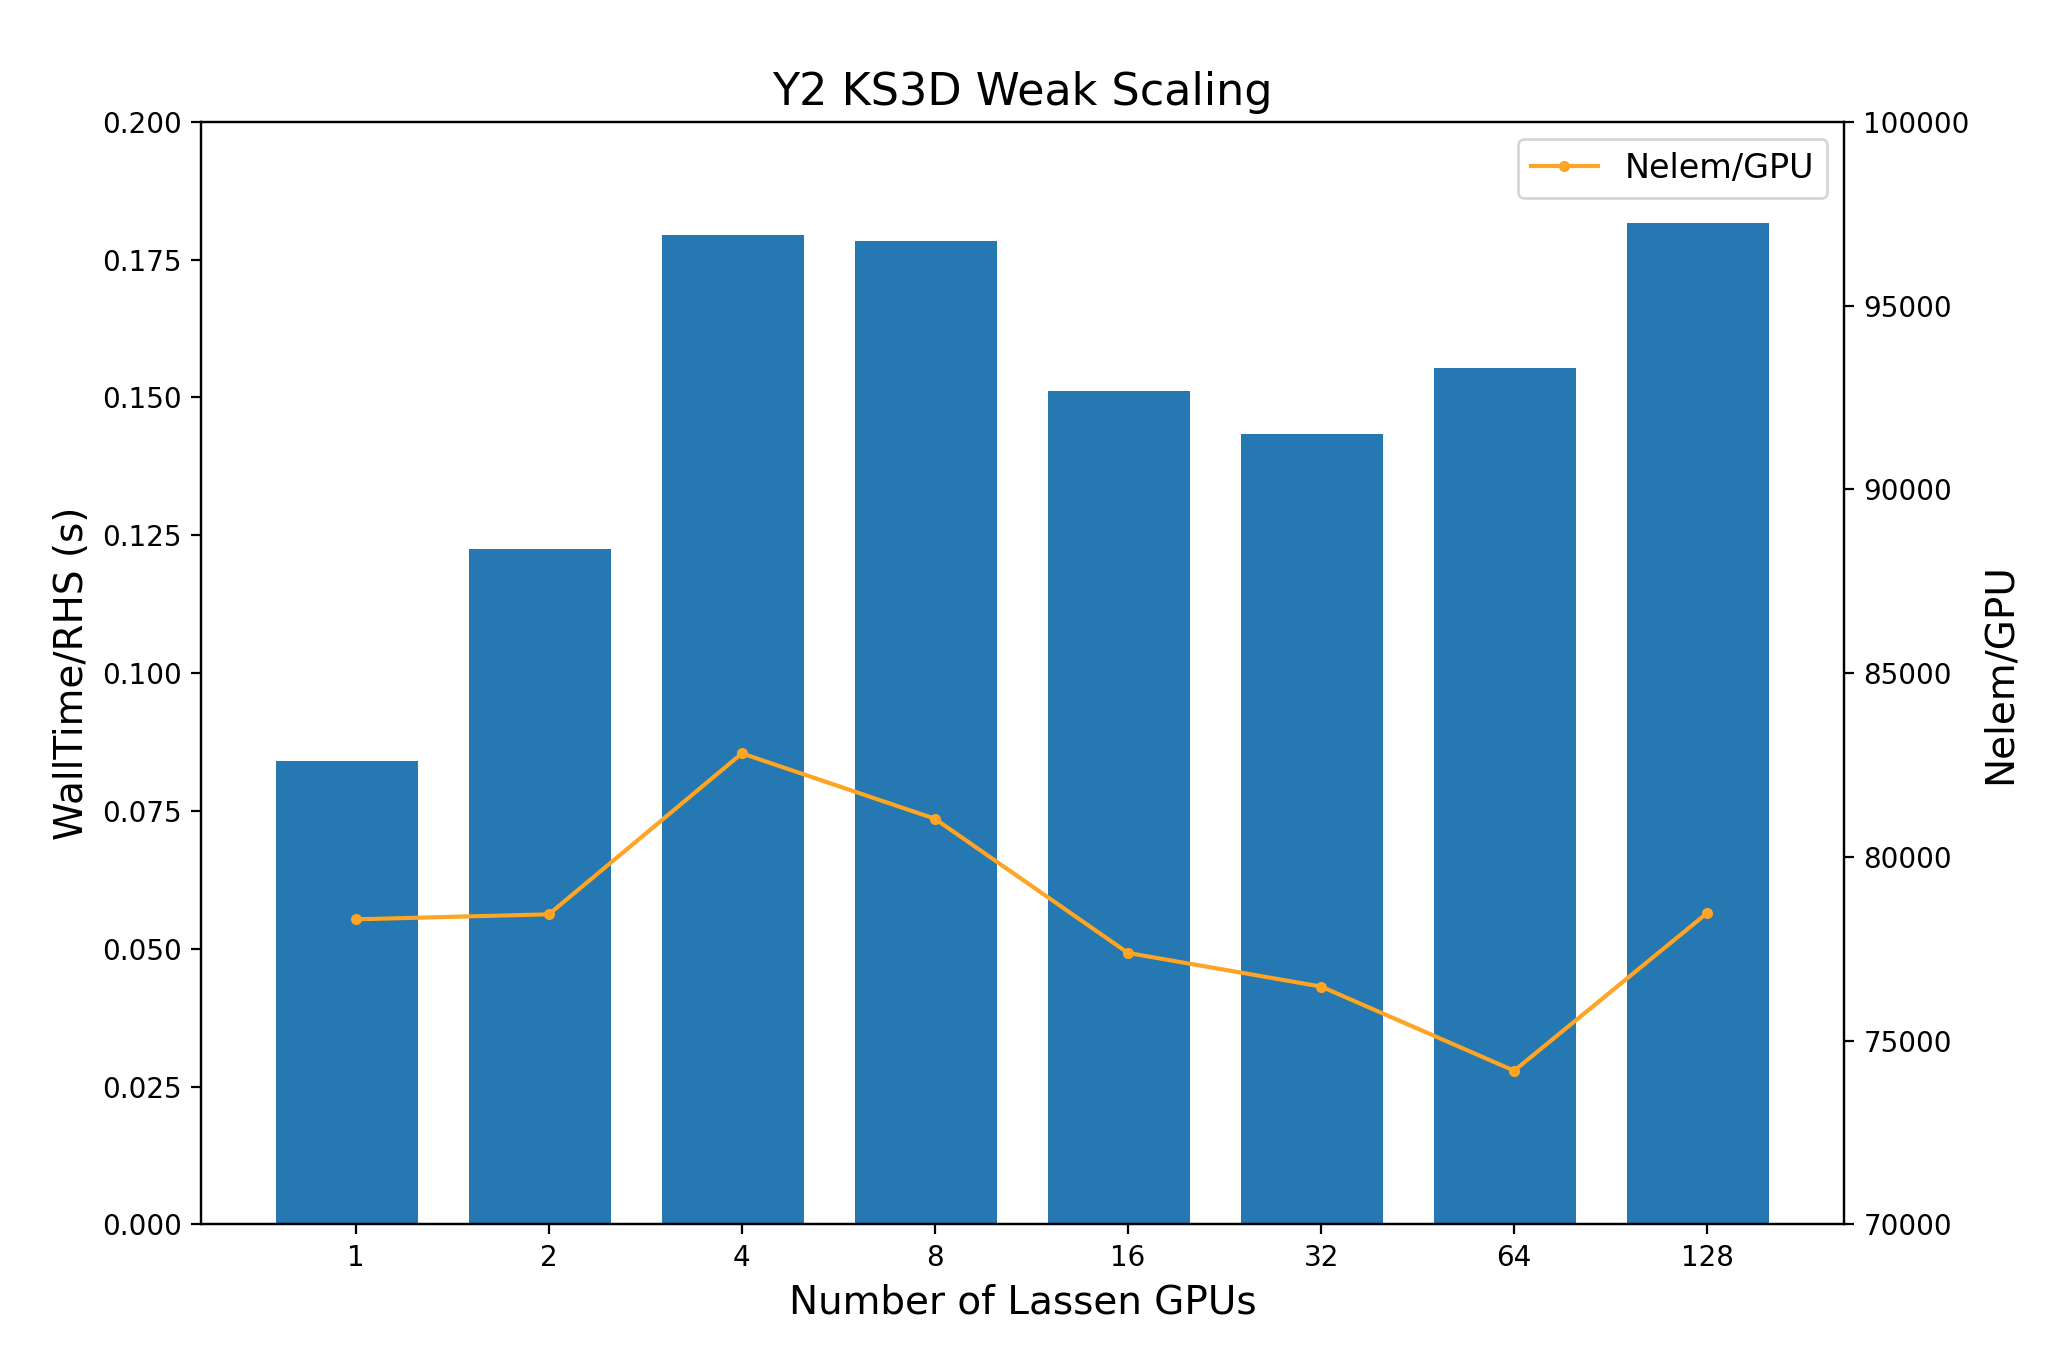
\includegraphics[width=.48\textwidth]{Figures/mtc/y2ks3d_weak.png}
%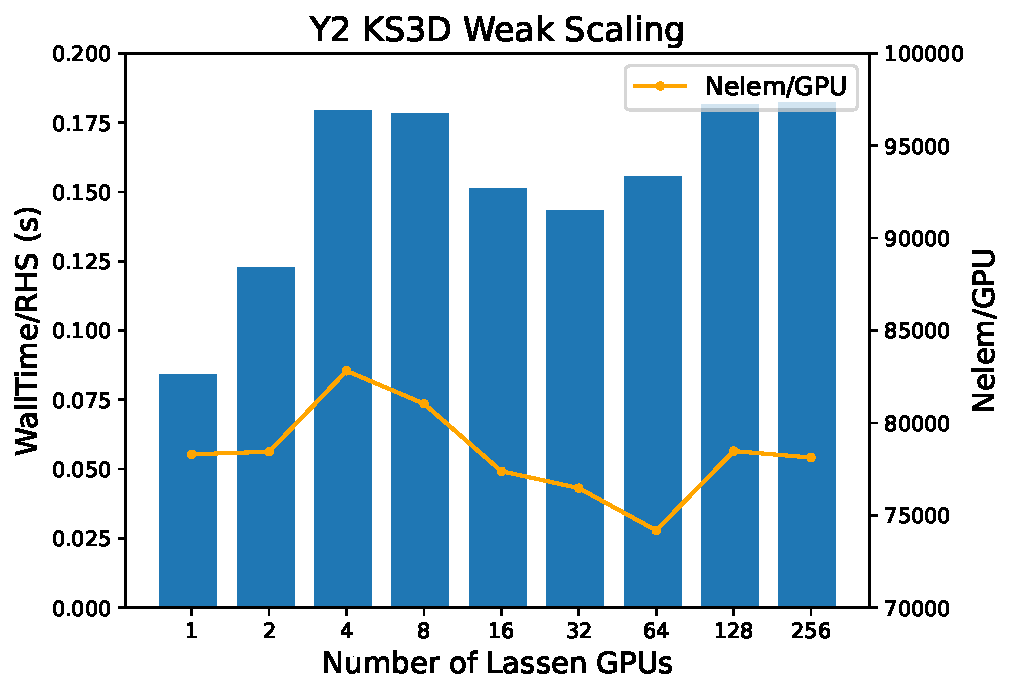
\includegraphics[width=.48\textwidth]{Figures/mtc/y2-prediction_weak_scaling.pdf}
%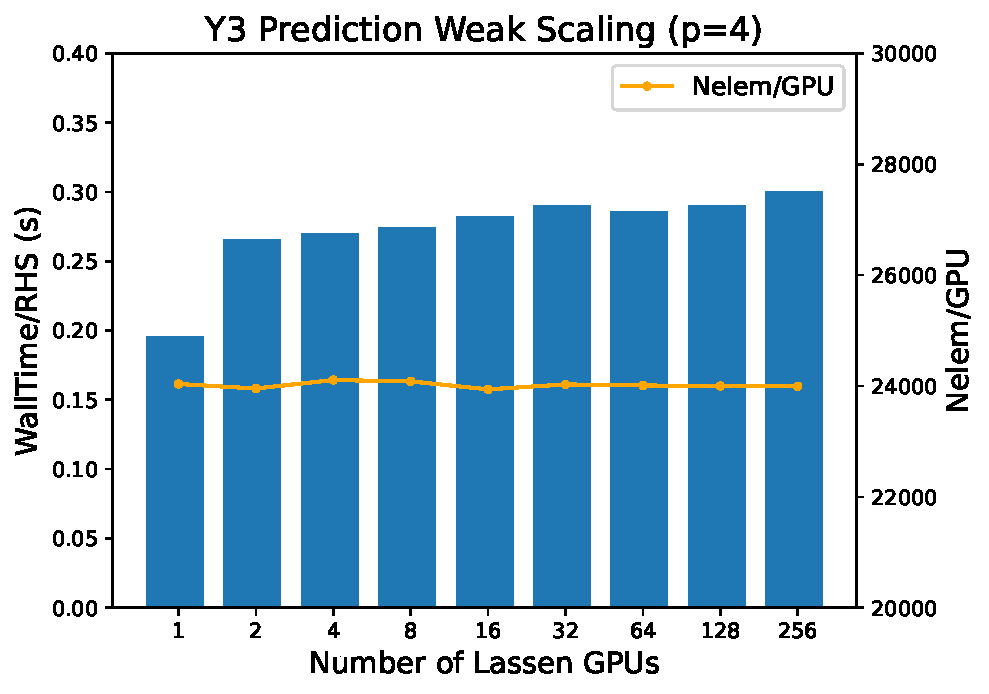
\includegraphics[width=.48\textwidth]{Figures/mtc/y3-prediction_weak_scaling.pdf}
%\end{minipage}
%\end{frame}

\begin{frame}\frametitle{Prediction Performance Snapshots: Lassen DAT}
    \begin{columns}[T]  % [T] is for top vertical alignment
    % Left Column
    \begin{column}{0.5\textwidth}
      % Top left: Text
      \begin{itemize}
        \item Weak scaling: 24k $p4$ per GPU
        \item Fluid: NS-only, 2 species
        \item AV: Fluid + Artificial Viscosity
        \item AVMix: AV + 7 species mixture EOS
        \item AVMixLimit: AVMix + species limiter
        \item FullPhysics: AVMixLimit + PLTransport + Wall
      \end{itemize}
      % Bottom left: RHS Compile Times
      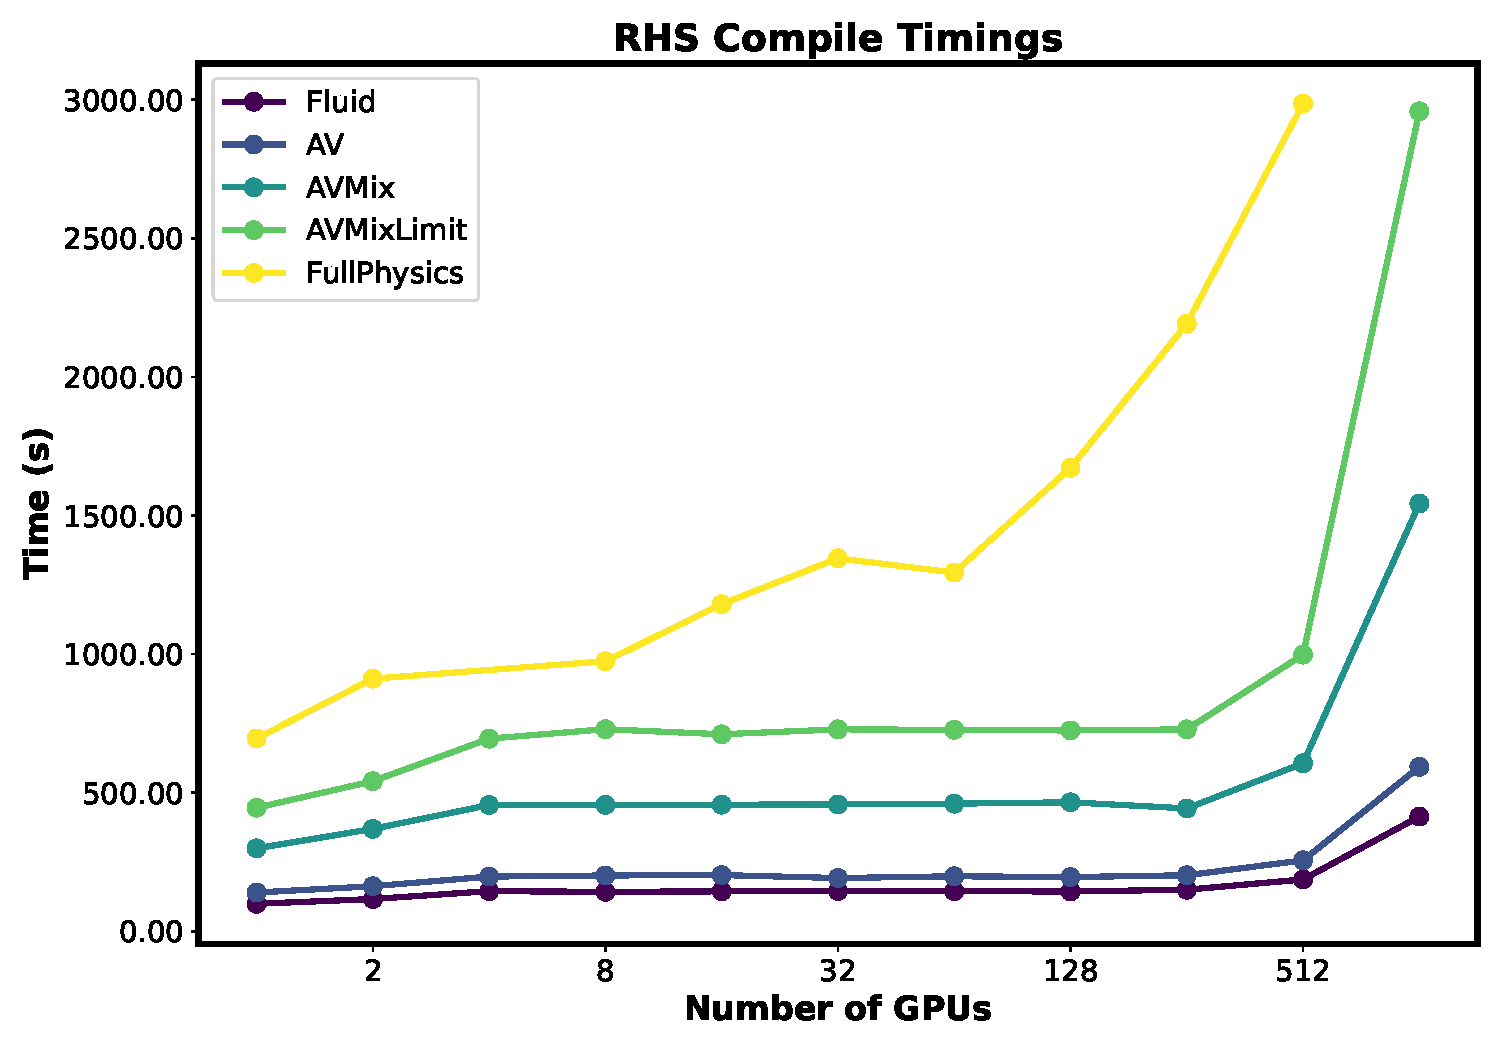
\includegraphics[width=.7\textwidth]{Figures/RHSCompileTimes.pdf}
    \end{column}
    
    % Right Column
    \begin{column}{0.5\textwidth}
      % Top right: Startup Times
      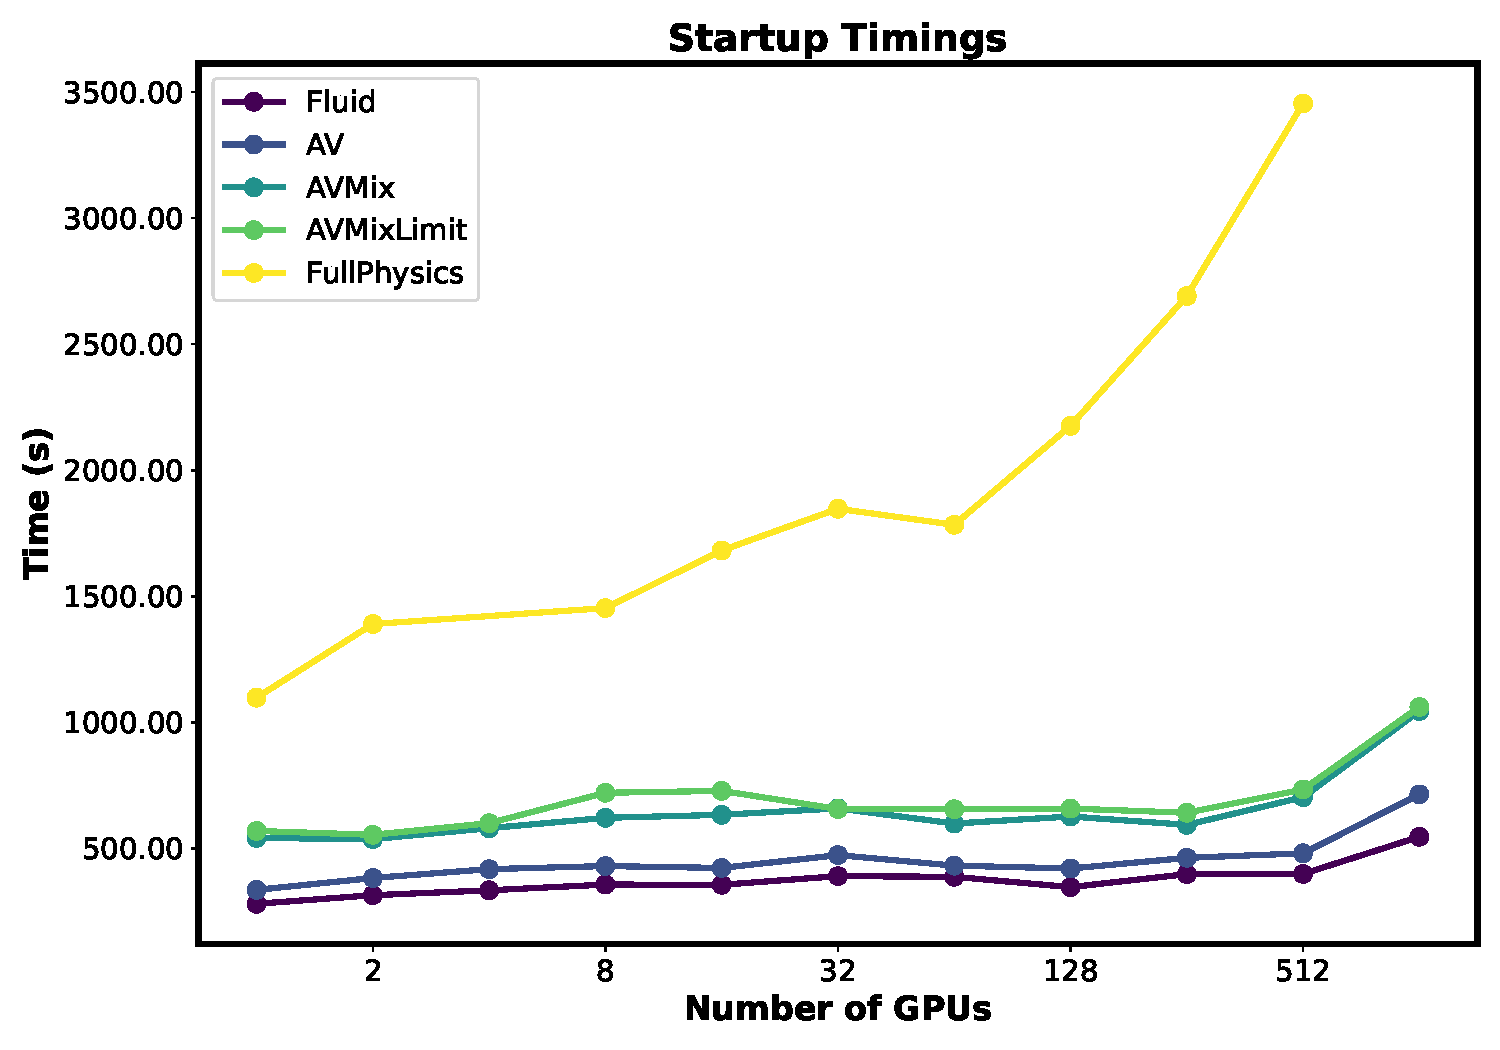
\includegraphics[width=.7\textwidth]{Figures/StartupTimes.pdf}
      % Bottom right: Simulation Step Times
      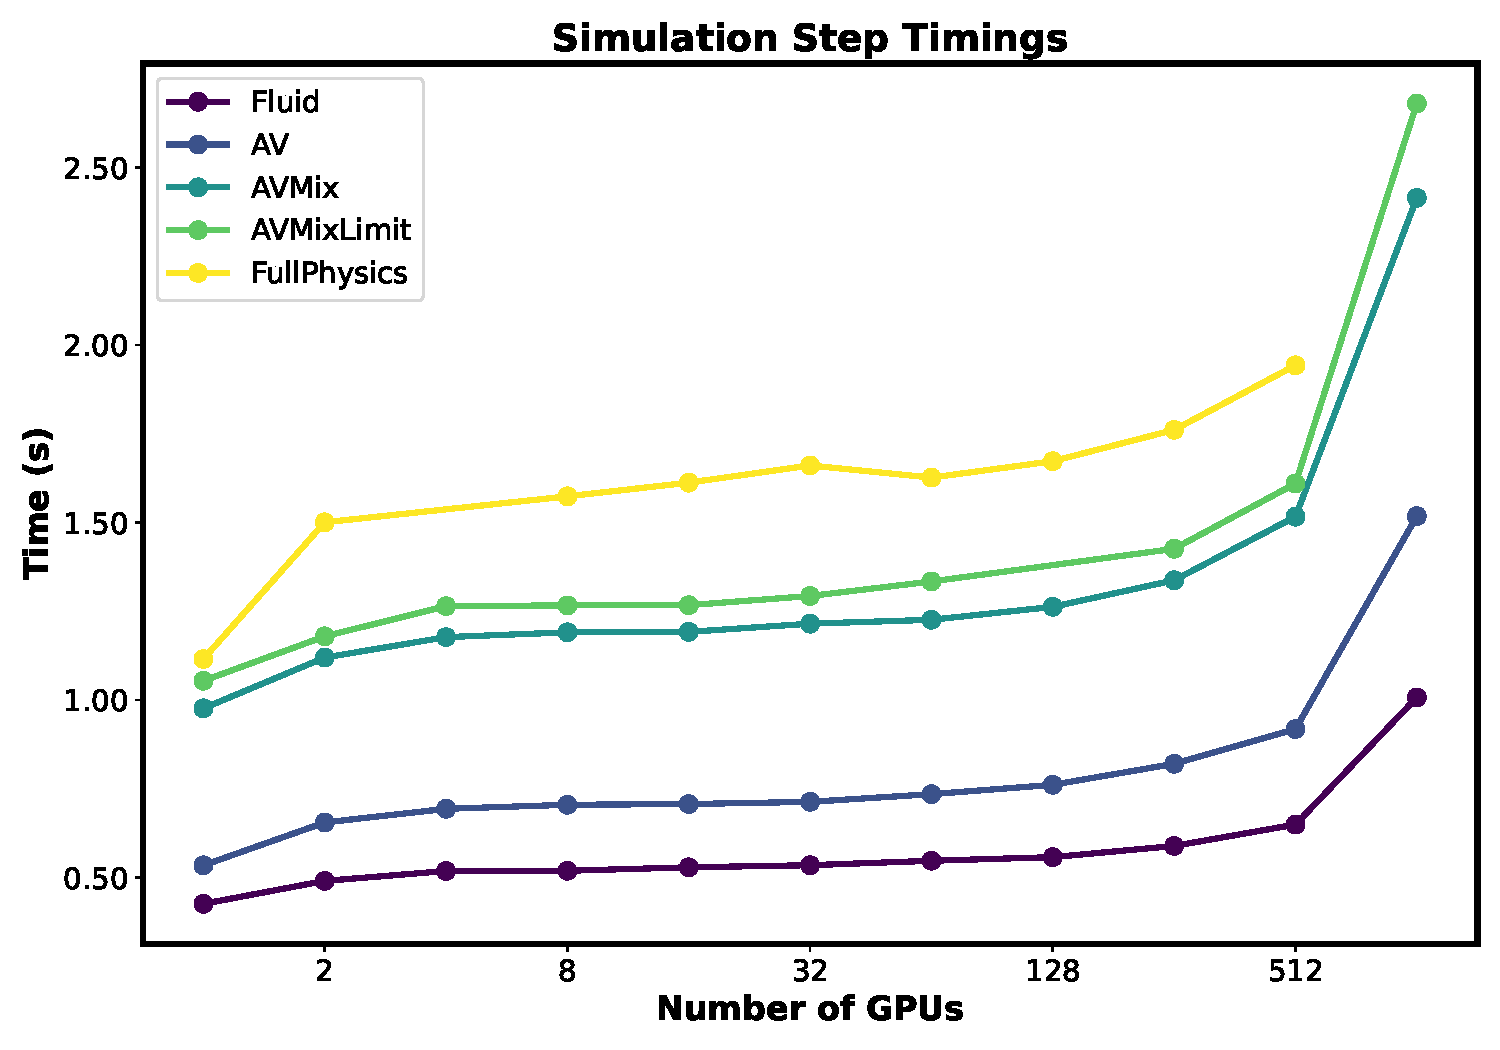
\includegraphics[width=.7\textwidth]{Figures/SimulationStepTimes.pdf}
    \end{column}
  \end{columns}
\end{frame}

\begin{frame}\frametitle{DAG Splat Rises Again: No Surprises}
    \begin{columns}[T]  % [T] is for top vertical alignment
    % Left Column
    \begin{column}{0.5\textwidth}
      % Top left: Text
      \begin{itemize}
      %\item DAG Splat is the culprit for full machine scaling fail
      \item 1D Partitioning fails spectacularly at scale
      \item Pancakes $\rightarrow$ waffles
      \item Material-material interfaces contribute significantly to DAG
      \item Function outlining to the rescue!  (Soon!)
      \end{itemize}
      \vspace{20pt}
      \hspace{20pt}
      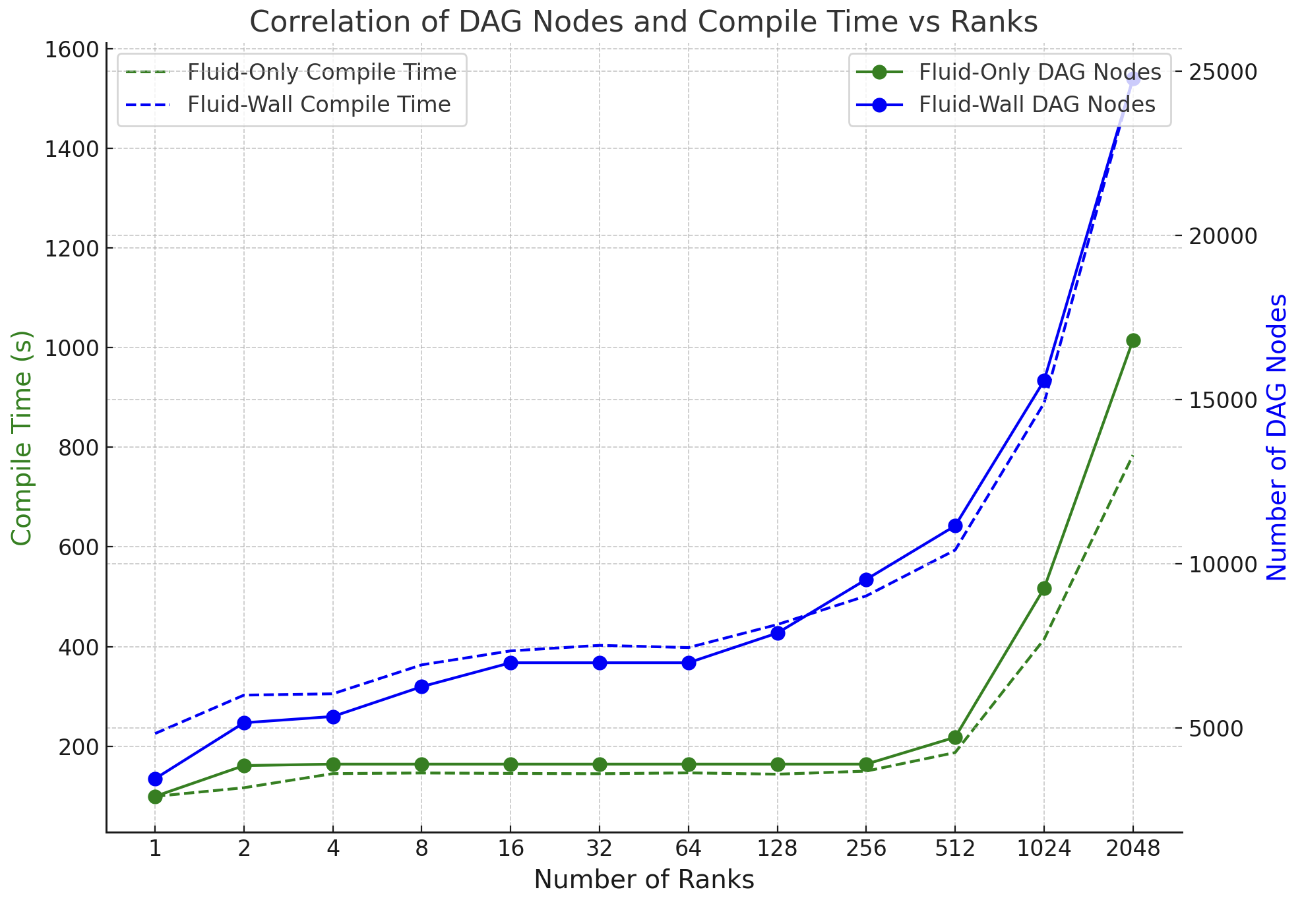
\includegraphics[width=.7\textwidth]{Figures/mtc/compile_times_dag_nodes.png}
    \end{column}
    
    % Right Column
    \begin{column}{0.5\textwidth}
      \vspace{-15pt}
      \hspace{60pt}
      % Top right: Startup Times
      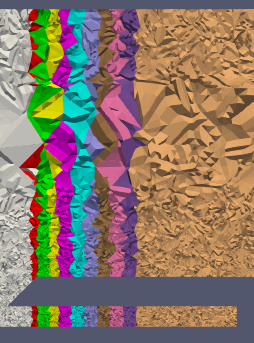
\includegraphics[width=.4\textwidth]{Figures/mtc/BadPartitioning.png}
      % \includegraphics[width=.7\textwidth]{Figures/mtc/StartupTimes_2048.png}
      % Bottom right: Simulation Step Times
      \vfill
      \vspace{10pt}
      \hspace{20pt}
      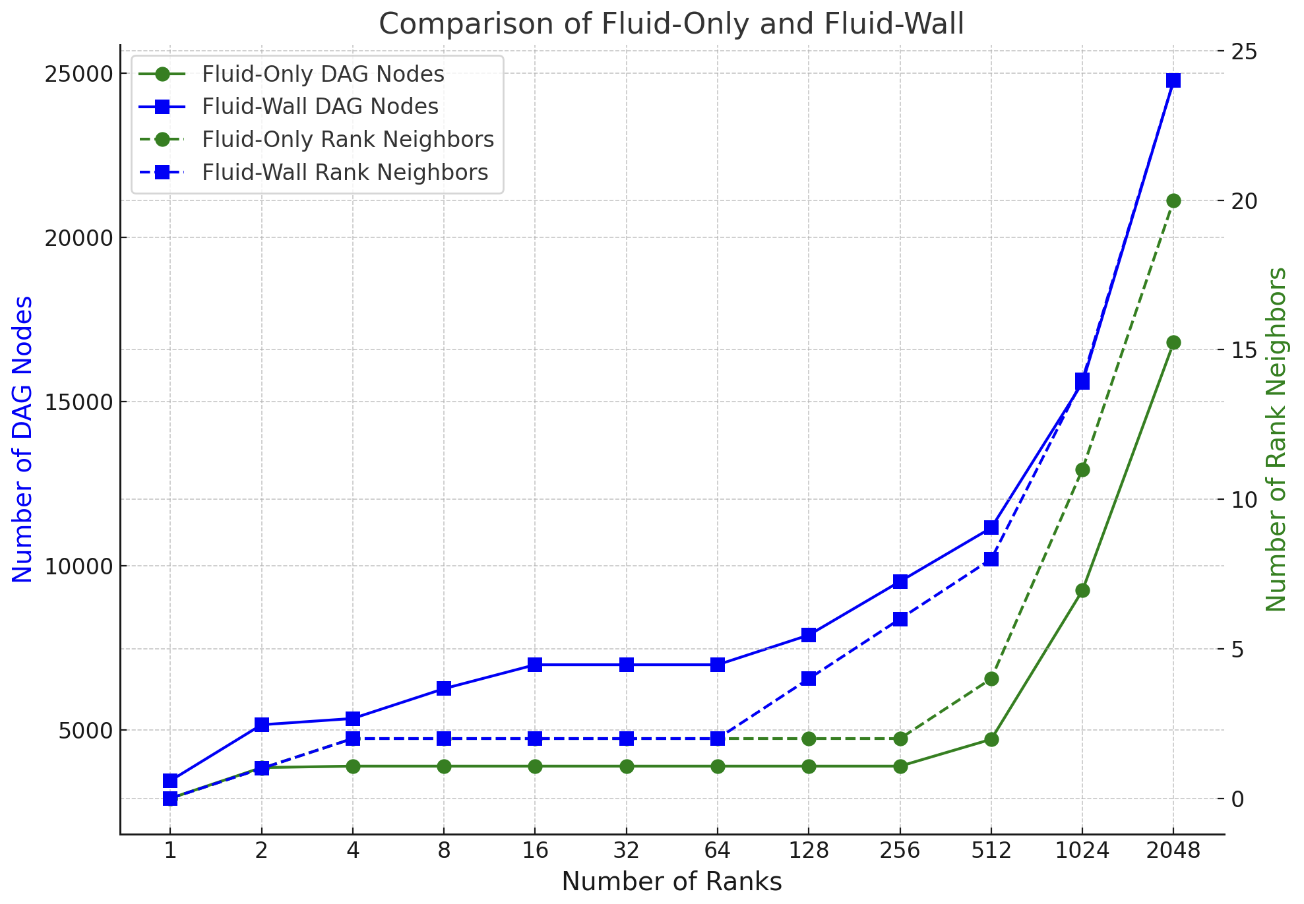
\includegraphics[width=.7\textwidth]{Figures/mtc/dag_nodes_rank_nbrs.png}
    \end{column}
  \end{columns}
\end{frame}

%\begin{frame}\frametitle{Prediction Performance Snapshots}
%\end{frame}

%\begin{frame}\frametitle{Prediction Performance Snapshots}
%\end{frame}


% - PLANS CHANGE
%\begin{frame}\frametitle{Developments for Y3 Prediction}
%\begin{center}
%Y3 Driver\\
%https://github.com/illinois-ceesd/drivers\_y3-prediction
%\end{center}
%\begin{multicols}{2}
%\begin{itemize}
%\item Kitchen sink (KS) feature set
%  \begin{itemize}
%  \item Coupled CNS + Wall/heat
%  \item Ethylene mixture, reaction sources, species limiting, power-law transport
%  \item Wall degradation, oxygen diffusion, reactive/porous mat.
%  \item Artificial physical viscosity, and sponge
%  \item OFF: Mixture transport, spectral filtering on RHS
 % \end{itemize}
%\item Meshes: 2D/3D updated geom, 2 test sects., shallower cavity
%\item Sims: 3D coupled (6M,p=4 256 GPUs), and smaller
%\item Scalability scripting and inputs (@add-scalability)
%\end{itemize}
%\end{multicols}
%\end{frame}

%\begin{frame}\frametitle{Path to Y3 Prediction}
%\begin{multicols}{2}
%\begin{itemize}
%\item Physics and modeling: Radiation \& Phenolics (mild gap)
%\item Numerics and discretization
%  \begin{itemize}
%  \item Mesh modifications (upstream injector, possible refinement)
%  \item Maybe (gaps suspected):
%    \begin{itemize}
%    \item Higher order mesh + filtering (likely!)
%    \item New AV
%    % \item Slope limiters
%    \item Multi-order meshes/volumes
%    \item ESDG? \prj{\tiny}{Zirui Wang}
%    \item Stop gap: High viscosity, maybe reduced physics
%    \end{itemize}
%  \end{itemize}
%\columnbreak
%\item Performance - closing gaps
%  \begin{itemize}
%  \item Cost per step (inert, comb): (.5, 1.4)s
%  \item Sim time: 1ms inert, 6e-4 w/comb
%  \item Estimated DT: .5ns
%  \item 12d inert, 19d comb
%  \item Any improvements welcomed
%  \end{itemize}
%\end{itemize}
%\end{multicols}
%\end{frame}

%\begin{frame}\frametitle{Path to Y3 Prediction}
%\begin{center}
%\item Preparing for prediction runs
%\end{center}
%\begin{multicols}{2}
%\begin{itemize}
%\item 3M(ish) 3D p=3 elems 
%\item Potentially serious issues: Shock/boundary, fluid/material
%\item Investigating higher order, with filtering, high visc
%\item Many scoping, physics-targeted, and debugging runs
%\end{itemize}
%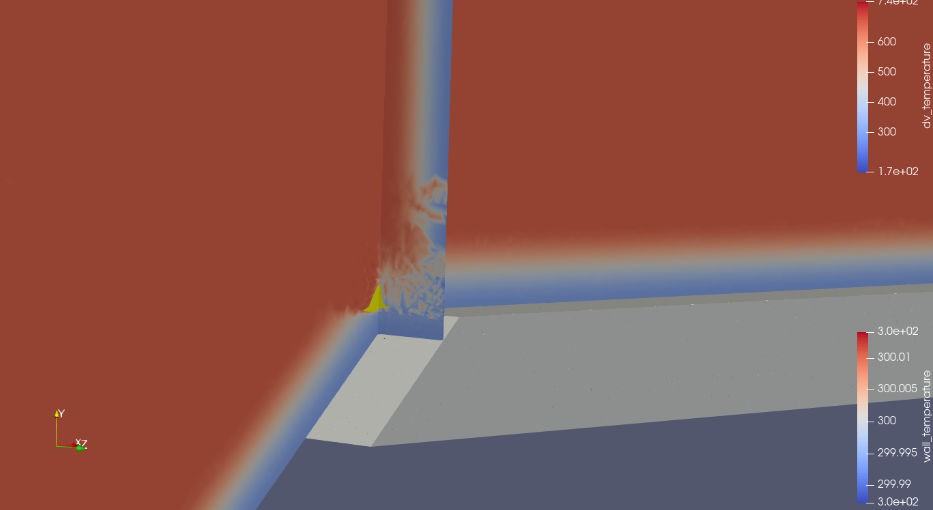
\includegraphics[width=.3\textwidth]{Figures/mtc/hot_edge.png}
%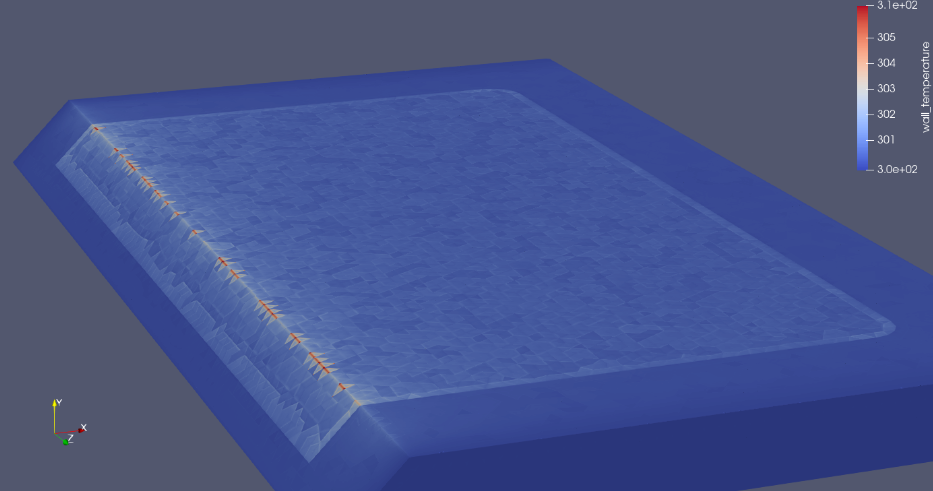
\includegraphics[width=.4\textwidth]{Figures/mtc/3d_yellow_cells.png}
%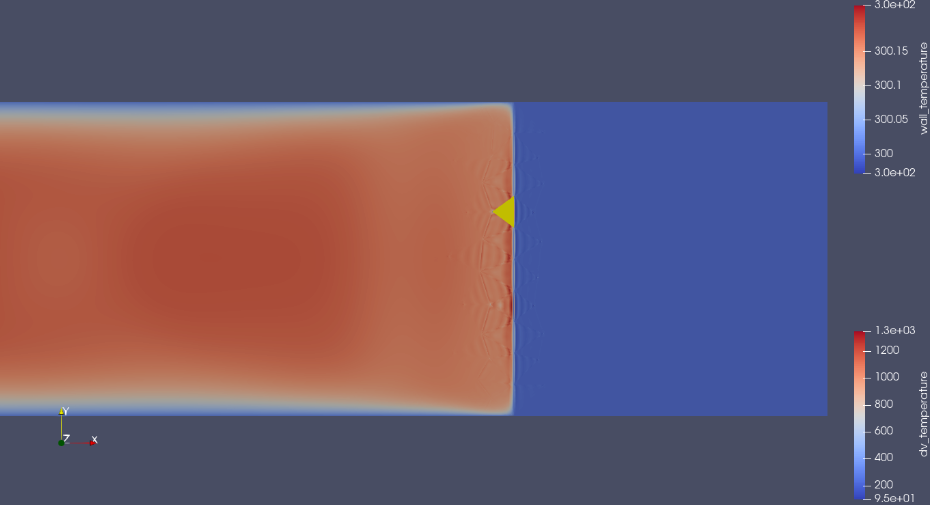
\includegraphics[width=.4\textwidth]{Figures/mtc/2d_yellow_cells.png}
%\end{multicols}
%\end{frame}

%\begin{frame}\frametitle{Path to Y3 Prediction}
%\begin{multicols}{2}
%\begin{itemize}
%\item Some pain points
%  \begin{itemize}
%  \item Transfinite or ultra fine mesh to stabilize fluid boundary
    % \begin{itemize}
    % \item Increases complexity of meshing by a lot
    % \item Increases number of elements
    % \item Hex support desired, might help
    % \end{itemize}
%  \item Lack confidence in correctness of model implementation
    % \begin{itemize}
    % \item Problem with numerics, or defect?
    % \item More extensive testing!
    % \item More experience/intuition about the numerics
    % \item ESDG?, FV?
    % \end{itemize}
%  \item Small problem performance is a drag
    % \begin{itemize}
    % \item 20m compile (this is fine, not fine)
    % \item DAG splat elim, faster compile
    % \end{itemize}
%  \item Makes lots of big files
    % \begin{itemize}
    % \item PARSL
    % \item Viz Driver
    % \end{itemize}
%  \item Development and testing viscosity
%  \item Long queues on available platforms
%  \item Cannot change size of run to adapt to resources
%  \end{itemize}
%\end{itemize}
%\end{multicols}
%\end{frame}


%\begin{frame}\frametitle{Near-term Development Outlook}
%\begin{multicols}{2}
%\begin{itemize}
%\item Now
%  \begin{itemize}
%  \item Understanding performance (why is it hard?)
%    \begin{itemize}
%    \item Code $\leftrightarrow$ Kernel \prj{\tiny}{M.~Diener}
%    \item Performance model
%    \item Kernel rooflines \prj{\tiny}{Nick Christensen}
%    \item Feature-specific
%    \end{itemize}
%  \item Evaluate Tioga
%  \item Boundary verif (MMS)
%  \item PARSL for testing \prj{\tiny}{D.~Friedel}
%  \end{itemize}
%\end{itemize}
%\columnbreak
%\begin{itemize}
%\item For prediction: (4mo horizon)
%  \begin{itemize}
%  \item Radiation \& phenolics \prj{\tiny}{T.~Ricciardi, M.~Smith}
%  \item \sout{DAG splat} \prj{\tiny}{Kaushik Kulkarni}
%  \item Mechanism parameterization for UQ
%  \item PARSL for UQ \prj{\tiny}{D.~Friedel}
%  \item Stabilizing prediction runs \prj{\tiny}{M.~Anderson}
%    \begin{itemize}
%    \item ESDG \prj{\tiny}{Zirui Wang}
%    \item Mixed-order
%    \item Quad/Hex support \prj{\tiny}{Addison Alvey-Blanco}
%    \item Curvlinear elements
%    \end{itemize}
%  \end{itemize}
%\end{itemize}
%\end{multicols}
%\end{frame}

%\begin{frame}\frametitle{Nice to have any time}
%\begin{multicols}{2}
%\begin{itemize}
%\item Reducing prediction pain (important):
%  \begin{itemize}
%  \item Reduce technical debt (merges)
%  \item Driver unification
%  \item Help with mesh generation
%  \item Visualization driver
%  \item PARSL for queue management
%  \item M-to-N restart
 % \end{itemize}
%%\item Potentially high-impact performance improvements
%  \begin{itemize}
%  \item Kernel Autotuning \prj{\tiny}{Nick Christensen}
%  \item Node-aware communication \prj{\tiny}{Shelby Lockhart}
%  \item DAG/compile time improvements \prj{\tiny}{Kaushik Kulkarni, M.~Diener}
%  \item Instrumentation (Mem \& Tags) \prj{\tiny}{Kaushik Kulkarni, M.~Diener}
%  \end{itemize}
%\item Future sims
%  \begin{itemize}
%  \item Mesh motion (interface regression)
%  \item Wall degradation
%  \item Turbulence modeling
%  \end{itemize}
%\end{itemize}
%\end{multicols}
%\end{frame}

